In this section, we introduce the combinatorial and diagrammatic replacements for both sides of the Quantum Geometric Satake functor: the category $\cwebs$ of webs, describing $\Fund_q^{\Om} \subset \Rep^{\Om}(U_q(\mathfrak{sl}_n))$, and the category $\DiagSBS$ of singular Soergel diagrams, describing $\SBSBim \subset \SSBim$. We then  describe the Quantum Geometric Satake $2$-functor in \cref{subsec the functor} and address fullness and faithfulness in \cref{subsec fullness and faithfulness}, while also showing that it categorifies the reformulated Satake isomorphism. 
The proof that this $2$-functor is well-defined will be postponed to \cref{sec well-defined-ness of the functor}. See \cref{thm main} for a summary of the key results.



%==========================================================================
\subsection{The fundamental subcategory}\label{subsec the fundamental subcategory}
%==========================================================================

\begin{defn} Let $\Fund_q = \Fund_q(\mathfrak{sl}_n)$) denote the full monoidal subcategory of $\Rep_q = \Rep(U_q(\mathfrak{sl}_n))$ monoidally generated by the fundamental representations. It is a $\Q(q)$-linear category for a formal variable $q$ (though not an additive category, as we have not included direct sums). \end{defn}

The objects of $\Fund$ correspond to fundwords, in the sense of \cref{defn:fundword}. The Karoubi envelope of $\Fund_q$ is $\Rep_q$. Had we defined the analogous category over specializations of $\Z[q,q^{-1}]$ to other fields, the Karoubi envelope of $\Fund_q$ would agree with the category of tilting modules over that field.

As explained in \cref{subsec Satake Hecke algebroid}, $\Rep_q$ is an $\Om$-graded monoidal category, corresponding to which we constructed a 2-category $\qRep$ in \cref{defn- qRep Omega}. Being a full monoidal subcategory of $\Rep_q$, $\Fund_q$ is an $\Om$-graded-monoidal category as well. Now we define the corresponding sub-2-category of $\qRep$.

% We have the full monoidal subcategory $\Fund(\mathfrak{sl}_n)$ of $\Rep(\mathfrak{sl}_n)$ monoidally generated by the fundamental representations, such that the Karoubi envelope of $\Fund(\mathfrak{sl}_n)$ is $\Rep(\mathfrak{sl}_n)$. 
% Similarly, when $q$ is not a root of unity, we have a monoidal full subcategory $\Fund_q(\mathfrak{sl}_n)$ of $\Rep(U_q(\mathfrak{sl}_n))$ whose Karoubi envelope is $\Rep(U_q(\mathfrak{sl}_n))$.
% Being a full monoidal subcategory of $\Rep(U_q(\mathfrak{sl}_n))$, $\Fund_q(\mathfrak{sl}_n)$ is an $\Om$-graded-monoidal category as well, and one can construct a sub-2-category $\qFund$ of $\qRep$ from this category.

\begin{definition}\label{defn- qFund Omega}
 The $2$-category $\qFund$ is defined as follows:
  \begin{itemize}
      \item The set of objects is $\Omega$.
      \item The Hom-category $\Hom(l,k)$ is defined as $\Fund_q^{k-l} := \Rep(U_q(\mathfrak{sl}_n))^{k-l} \cap \Fund_q$.
\end{itemize}
    % \item Composition of 1-morphisms is given by tensor product of representations.
      
      % For $s\in \tilde{\Theta}$ and $\omega \in \Om$, the $\Hom$-category $\Hom(s,s\omega)=\Fund_q(\mathfrak{sl}_n)\cap \Rep(U_q(\mathfrak{sl}_n))^\omega$. 
\end{definition}

In other words, $\qFund$ is a 2-full sub-2-category of $\qRep$ where the 1-morphisms are generated monoidally by the fundamental representations. The $1$-morphisms of $\qFund$ correspond to colored fundwords in the sense of \cref{def:GSfundword}.

%==========================================================================
\subsection{Colored \texorpdfstring{$\mathfrak{sl_n}$}{sl\_n}-Webs}\label{subsec-colored sln webs}
%==========================================================================

% In this section, we discuss the diagrammatic presentation for $\Fund_q(\mathfrak{sl}_n)$ and for $\qFund$ in terms of \emph{$\mathfrak{sl}_n$-webs} and \emph{colored $\mathfrak{sl}_n$-webs} respectively.

A diagrammatic presentation for $\Fund_q(\mathfrak{sl}_n)$ over $\C(q)$ was first given by Cautis--Kamnitzer--Morrison in \cite{CKM}. In this paper, we use a different presentation from work of Bigelow \cite{Bigelow}, where the base field is also assumed to be $\C(q)$.  More accurately, both \cite{CKM} and \cite{Bigelow} describe a category which is larger than $\Fund_q$, having as generating objects both the fundamental representations and their duals. However, $\Fund_q$ is equivalent to this larger category (the inclusion functor is essentially surjective), as the duals of fundamental representations are isomorphic to other fundamental representations. Diagrammatically, these isomorphisms are drawn as tags.

In \cite[Proposition 1]{Bigelow}, Bigelow shows that the web relations in \cite{CKM} follow from this smaller collection of relations over $\C(q)$, and the proof only requires that the quantum integers are invertible. In particular, the proofs in \cite{CKM} and \cite{Bigelow} both work over $\Q(q)$.

Bigelow's relations are those shown in \cref{fig:webrel}, up to taking mirror images and arrow reversals. While the generating morphisms in Bigelow's presentation look the same as in Cautis--Kamnitzer--Morrison's presentation, the meaning of some of the generating morphisms is different; they have different conventions for the ``tag.'' In particular, Bigelow's tags are defined in such a way that his webs admit both reflection symmetry and arrow reversal symmetry. The webs in \cite{CKM} are invariant under simultaneously reflecting and reversing arrows, but not under either individual operation.

\begin{remark} Bigelow ``fixes'' a subtle sign error in \cite{CKM}. The relations explicitly written in \cite{CKM} are correct, but the paper incorrectly asserts that the orientation-reversed relations also hold; this fails for equations (2.7) and (2.8) therein, being off by a sign, as Bigelow observed.  \end{remark}

\begin{definition}\label{defn-webs}
    The category of (Bigelow-style) $\mathfrak{sl}_n$-webs, denoted $\Webs$, is defined as follows.
    \begin{itemize}
        \item The objects are generated monoidally by oriented points labelled by $i\in\set{1,2, \ldots, n-1}$.
        \item The morphisms are generated ($\Q(q)$-linearly) by clockwise and counter-clockwise cups and caps, along with bivalent vertices (tags) and trivalent vertices as shown below:
        \[
            \begin{array}{OOOO}
        \phantom{ \tikz[x=1mm, y=1mm, baseline=-0.5ex]{\draw (0,-10) -- (0,10)}} %for vertical spacing
         \tikz[x=1mm,
         y=1mm,
         baseline=-0.5ex] {
          \draw[->-] (0,-5) arc (0:180:5) node [pos=0.5, above] {$k$};
        } 
        &
        \tikz[x=1mm,
         y=1mm,
         baseline=-0.5ex] {
          \draw[-<-] (0,-5) arc (0:180:5) node [pos=0.5, above] {$k$};
        } 
        &\tikz[x=1mm,
         y=1mm,
         baseline=-0.5ex] {
          \draw[->-] (0,5) arc (180:360:5) node [pos=0.5, below] {$k$};
        } 
        &\tikz[x=1mm,
         y=1mm,
         baseline=-0.5ex] {
          \draw[-<-] (0,5) arc (180:360:5) node [pos=0.5, below] {$k$};
        } 
        \\
        \phantom{ \tikz[x=1mm, y=1mm, baseline=-0.5ex]{\draw (0,-10) -- (0,10)}} %for vertical spacing
        \tikz[x=1mm,
         y=1mm,
         baseline=-0.5ex] {
          \draw[->-] (0,0) -- (0,6) node [above] {$k$};
          \draw[->-] (0,0) -- (0,-6) node [below] {$n - k$};
          \draw (0,0) -- (2,0);
        } 
        & 
        \tikz[x=1mm,
         y=1mm,
         baseline=-0.5ex] {
          \draw[-<-] (0,0) -- (0,6) node [above] {$k$};
          \draw[-<-] (0,0) -- (0,-6) node [below] {$n - k$};
          \draw (0,0) -- (2,0);
        }
        &
        \tikz[x=1mm, y=1mm, baseline=-0.5ex] {
        \draw[->-] (-6,-6) node [below] {$k$}
          .. controls (-5,-5) and (-3,-3) .. (0,0);
        \draw[->-] (6,-6) node [below] {$l$}
          .. controls (5,-5) and (3,-3) .. (0,0);
        \draw[->-] (0,0) -- (0,6) node[above]{$k+l$};
        }
        &
        \tikz[x=1mm, y=1mm, baseline=-0.5ex] {
        \draw[->-] (0,-6) node[below]{$k+l$} -- (0,0);
        \draw[-<-] (-6,6) node [above] {$k$} -- (0,0);
        \draw[-<-] (6,6) node [above] {$l$} -- (0,0);
      }
            \end{array}
            \]
        
        \item The cups and caps satisfy the isotopy relations, making the category pivotal (see \cite[Chapter 2]{Morr07} for further details.)
        \item  The morphisms satisfy the relations in \cref{fig:webrel}, and their mirror images and arrow reversals.
        As in \cite{Bigelow}, we shall refer to these relations in \cref{fig:webrel} as ``tag switching", ``tag cancellation”, ``I = H", ``bursting a digon" and ``bursting a square" respectively (from top to bottom, left to right).
        \item It is convenient to also allow strands labeled $0$ or $n$, with the following convention for deleting them. Any trivalent vertex that had a strand labeled $0$ simply ceases to be a vertex. Any trivalent vertex that had a strand labeled $n$ becomes a bivalent vertex, with a tag on the side of the deleted strand.
        
    \end{itemize}
\end{definition}
\begin{figure}[h]
  \[
    \begin{array}{|T|T|}
      \hline
      % switch tag | cancel tags
      {
        \phantom{ \tikz[x=1mm, y=1mm, baseline=-0.5ex]{\draw (0,-10) -- (0,10)}} %for vertical spacing
        \tikz[x=1mm,
  y=1mm,
  baseline=-0.5ex] {
          \draw[->] (0,0) -- (0,6) node [right] {$k$};
          \draw[->] (0,0) -- (0,-6) node [right] {$n - k$};
          \draw (0,0) -- (2,0);
        }
        = (-1)^{k(n - k)} \tikz[x=1mm, y=1mm, baseline=-0.5ex]{
          \draw[->] (0,0) -- (0,6) node [right] {$k$};
          \draw[->] (0,0) -- (0,-6) node [right] {$n - k$};
          \draw (0,0) -- (-2,0);
        }
      } &
      {
        \tikz[x=1mm,
         y=1mm,
        baseline=-0.5ex] {
          \draw[->-] (0,-6) -- (0,-2);
          \draw (0,-2) -- (2,-2);
          \draw[->-] (0,2) -- (0,-2);
          \draw (0,2) -- (2,2);
          \draw[->] (0,2) -- (0,6) node [right] {$k$};
        }
        = \, \tikz[  x=1mm,
  y=1mm,
  baseline=-0.5ex] {
          \draw[->] (0,-6) -- (0,6) node [right] {$k$};
        }
      } \\ \hline
      % I=H  | digon
      {
        \phantom{ \tikz[x=1mm, y=1mm, baseline=-0.5ex] {\draw (0,-10) -- (0,10)}} %for vertical spacing
        \tikz[x=1mm, y=1mm, baseline=-0.5ex] {
          \draw[->-] (-6,-6) node [left] {$l$}
            .. controls (-5,-5) and (-4,-3) .. (0,-3);
          \draw[->-] (6,-6) node [right] {$m$}
            .. controls (5,-5) and (4,-3) .. (0,-3);
          \draw[->-] (0,-3) -- (0,3);
          \draw[->-] (-6,6) node [left] {$k$}
            .. controls (-5,5) and (-5,3) .. (0,3);
          \draw[->] (0,3) .. controls (4,3) and (5,5) .. (6,6);
        }
        = \tikz[x=1mm, y=1mm, baseline=-0.5ex] {
          \draw[->-] (-6,-6) node [left] {$l$}
            .. controls (-5,-5) and (-3,-4) .. (-3,0);
          \draw[->-] (-6,6) node [left] {$k$}
            .. controls (-5,5) and (-3,4) .. (-3,0);
          \draw[->-] (-3,0) -- (3,0);
          \draw[->-] (6,-6) node [right] {$m$}
            .. controls (5,-5) and (3,-4) .. (3,0);
          \draw[->] (3,0) .. controls (3,4) and (5,5) .. (6,6);
        }
      } &
      {
        \tikz[x=1mm, y=1mm, baseline=-0.5ex] {
          \draw[->-] (0,-8) -- (0,-4);
          \draw[->-] (0,-4) arc (270:90:4);
          \draw[->-] (0,-4) arc (-90:90:4) node[pos=0.5,right]{$1$};
          \draw[->] (0,4) -- (0,8) node [right] {$k$};
        }
        = [k] \: \tikz[x=1mm, y=1mm, baseline=-0.5ex] {
          \draw[->] (0,-8) -- (0,8) node [right] {$k$};
        }
      } \\ \hline
    % square
    \multicolumn{2}{|F|}
    {
      \phantom{ \tikz[x=1mm, y=1mm, baseline=-0.5ex] {\draw (0,-10) -- (0,10)}} %for vertical spacing
      \tikz[x=1mm, y=1mm, baseline=-0.5ex] {
        \draw[->-] (45:4) arc (45:135:4) node [pos=0.5, above]{$1$};
        \draw[-<-] (135:4) arc (135:225:4);
        \draw[->-] (225:4) arc (225:315:4) node [pos=0.5, below]{$1$};
        \draw[->-] (315:4) arc (315:405:4);
        \draw[->-] (7,-7) node [right] {$1$} -- (315:4);
        \draw[->] (45:4) -- (7,7) node [right] {$1$};
        \draw[->] (135:4) -- (-7,7) node [left] {$k$};
        \draw[->-] (-7,-7) node [left] {$k$} -- (225:4);
      }
      =
      \tikz[x=1mm, y=1mm, baseline=-0.5ex] {
        \draw[->-] (-7,-7) node [left] {$k$}
          .. controls (-6,-6) and (-3,-5) .. (0,-4);
        \draw[->-] (7,-7) node [right] {$1$}
          .. controls (6,-6) and (3,-5) .. (0,-4);
        \draw[->-] (0,-4) -- (0,4);
        \draw[->] (0,4) .. controls (-3,5) and (-6,6)
          .. (-7,7) node [left] {$k$};
        \draw[->] (0,4) .. controls (3,5) and (6,6)
          .. (7,7) node [right] {$1$};
      }
      + [k - 1] \tikz[x=1mm, y=1mm, baseline=-0.5ex] {
        \draw[->] (-7,-7) .. controls (-4,-4) and (-4,4)
          .. (-7,7) node [left] {$k$};
        \draw[->] (7,-7) .. controls (4,-4) and (4,4)
          .. (7,7) node [right] {$1$};
      }
    } \\ \hline
\end{array}
\]
\caption{Web relations. Some labels are omitted, but can be deduced.}
\label{fig:webrel}
\end{figure}

% It was shown in \cite{ELLCC} that the set of relations in \cite{CKM} is sufficient when working over $\Z[q,q^{-1}]$ (whereas this is not true for Bigelow's presentation). The same is therefore true over any extension of $\Z[q,q^{-1}]$. In particular, by base change to any ring where quantum numbers are invertible, one can combine Bigelow's equivalence with \cite{ELLCC} and \cite{CKM} to deduce the following theorem.

\begin{theorem}\label{thm webs present Fund}
    There is a $\Q(q)$-linear equivalence $\Fund_q \to \Webs$ which is not surjective on objects, but is essentially surjective. There is a fully faithful $\Q(q)$-linear functor $\Webs \rightarrow \Rep_q$. The composition of these functors is the inclusion functor $\Fund_q \subset \Rep_q$.
\end{theorem}

\begin{proof}  An equivalence between Cautis-Kamnitzer-Morrison's web category and the full subcategory of $\Rep_q$ generated by fundamental representations and their duals was proven in \cite[Theorem 3.3.1]{CKM}. We merely restrict the inverse equivalence to $\Fund_q$, and translate the result through Bigelow's equivalence. \end{proof}

\begin{remark} The analogous result for any $\Z[q,q^{-1}]$-algebra, when using Cautis-Kamnitzer-Morrison's webs, was proven in \cite{ELLCC}. \end{remark}

% This result also holds for the analogous $A$-linear categories, for any $\Z[q,q^{-1}]$-algebra $A$ where the quantum numbers are invertible.

This diagrammatic description of $\Fund_q(\mathfrak{sl}_n)$ naturally provides a diagrammatic description of the associated 2-category $\qFund$.

\begin{definition}
The 2-category of \emph{colored $\mathfrak{sl_n}-webs$}, denoted $\cwebs$ is defined as follows:
\begin{itemize}
    \item The objects are elements of $\Om$. 
    These objects label the regions in diagrams. The region labels will be colored in gray.
    \item For each $a \in \Om$ and $i \in \set{1,2,\ldots, n-1}$, there are 1-morphisms $i \in \Hom(a, a+i)$ and $i^* \in \Hom(a, a-i)$ which generate the category monoidally.
    We draw the identity $2$-morphism of $i \in \Hom(a,a+i)$ as an upward arrow, and that of $i^* \in \Hom(a, a-i)$ as a downward arrow as shown below.
    \begin{equation*}
        \gr{a+i}\uparrow^{\blk{i}} \gr{a}, \qquad \qquad
        \gr{a-i}\downarrow^{\blk{i}} \gr{a}
    \end{equation*}
    \item The 2-morphisms are generated by clockwise and counter-clockwise cups and caps, along with bivalent vertices (tags) and trivalent vertices as shown below:
    \[\begin{array}{cccc}
      \isvg{0.15}{cap_webs_c}   &\isvg{0.15}{cap_webs_cc} &\isvg{0.15}{cup_webs_c} &\isvg{0.15}{cup_webs_cc} 
    \end{array}
    \]
    \[\begin{array}{cccc}
        \isvg{0.15}{tag_right_c} &\isvg{0.15}{tag_right_d}  &\isvg{0.15}{trivalent_vertex_up} &\isvg{0.15}{trivalent_vertex_down}
    \end{array}\]
    \item The 2-morphisms satisfy the relations in \cref{fig:webrel} and their mirror images and arrow reversals, for any allowed labeling of the regions (an upward arrow labelled $k$ should have a region $a+k$ to the left and $a$ to the right and so on). The cups and caps satisfy the isotopy relations as in \cref{isotopy}.
    \item Same conventions as in \cref{defn-webs} for deleting strands labeled $0$ or $n$.
\end{itemize}
\end{definition}

\begin{theorem}\label{theorem cwebs present qFund}
    There is a $\Q(q)$-linear $2$-functor $\Fund^\Omega_q \to \cwebs$ which is an equivalence; it is not surjective on $1$-morphisms, but is essentially surjective. There is a fully faithful $\Q(q)$-linear $2$-functor $\cwebs \rightarrow \Rep^\Omega_q$. The composition of these functors is the inclusion functor $\Fund^\Omega_q \subset \Rep^\Omega_q$.
\end{theorem}

\begin{defn} \label{defn:symmetries of webs} We define $2$-functors $\sigma, \rotation, \Upsilon_W, \reversal \colon \cwebs \to \cwebs$, the basic symmetries of this category.

On objects/region labels $\sigma$ sends $a \mapsto a+1$. Aside from this relabling, diagrams remain unchanged. This is a monoidal, covariant equivalence.

On objects $\rotation$ sends $a \mapsto a$, and it rotates all diagrams by 180 degrees. This is an antimonoidal, contravariant equivalence.

On objects $\Upsilon_W$ sends $a \mapsto -a$, and it flips each diagram vertically (i.e. reflecting across a horizontal axis). This is a monoidal, contravariant equivalence.

On objects $\reversal$ sends $a \mapsto -a$, and it reverses all the orientations in each diagram. This is a monodial, covariant equivalence.
\end{defn}

%==========================================================================
\subsection{Diagrammatics for Singular Bott-Samelson Bimodules}
\label{subsec-diagrammatics for frob hypercube}
\label{subsec-diagrammatic singular bott-samelson bimodules}
%==========================================================================

% \BE{Ok philip, I'm going to make you do this reorganizational work, noting that this more general approach would be good for your thesis.  Outline of what should be below:}\PT{Working on it now.}

%\BE{Say that you're going to construct the diagrammatic category built in EWSFrob as it applies to a Frealization. Point out that some parts of the construction rely on properties which were proven in REF TO LEMMA ABOUT STAR ETC, and that these properties will not be mentioned again. Don't mention them again}

%\BE{Don't bother to define Bimgr at all! WE already have SBSBim and this is the right algebraic target in our special case!!! No need to redefine the algebraic target, just define the diagrammatic category. When defining it, let the objects be singlestep expressions, and point out that they're monoidally generated by Ind and Res (for which you can use similar notation to the below but use $i \in I$, not $\gamma$). REplace all the $\gamma$ and $\gamma'$ with $i$ and $j$. Talk abut the generating diagrams and the functor to SBSBim and move earlier your examples from current section 5.4. If you want, before imposing any relations but isotopy, you can call this category $\DiagSBS^{pre}$. (The advantage to doing something like this is that functors from the pre category are easy, and rotational/color symmetries already hold from pre category to pre category, so that lets you check/deffine other relations using those symmetries.)}

%\BE{Do the EWSFrob relations. Put all the reidemiester II relations in one place. First do the oriented one, then the two non-oriented ones. Point out the special case of the distant one like so. When $i$ and $j$ are in different components of $Iij$, then $\Phi^+_{Iij} \setminus \Phi^+_{Ii} = \Phi^+_{Ij} \setminus \Phi^+_{I}$ so the $\mu$s are all 1, and (unoriented R2 eqref) reduces to (distant R2). (It's worth saying this aloud because the scalar depends on this kind of consistency.)   Then do the RIII moves in one place, oriented then unoriented then distant, but you don't need to spell it out as much for the distant one.}

%\BE{Then you can define the quotient $\DiagSBS$, and there's really no need for any discussion of additional relations! Eliminate section 5.4 having moved everything relevant here.}

% \BE{Then define $\sigma$ and $\Upsilon$ (optional: on both the pre and final category).}

% In this section, we fix a (graded) Frobenius hypercube $(\Gamma, \mc{F})$ and construct an algebraic category $\mc{C}(\Gamma)$, and a diagrammatic category $\mc{D}(\Gamma)$ associated to it, following \cite{EWSFrob}.

% \begin{defn} 
% %Let $\Bim$ denote the 2-category whose objects are algebras, where $\Hom_{\Bim}(A,B)$ is the category of $(B,A)$-bimodules which are finitely generated as left $B$-modules and as right $A$-modules. 
% Let $\Bimgr$ whose objects are graded algebras, where $\Hom_{\Bimgr}(A,B)$ is the category of graded $(B,A)$-bimodules which are finitely generated as left- and right- graded modules. The 2-morphisms are the graded Hom spaces as defined in \cref{defn- graded Hom}.
% Horizontal composition is given by tensor product. 
% Given a graded $(B,A)$-bimodule $M$, we sometimes write it as $\Bimod{B}{A}{M}$ to
% emphasize which algebras act on it. 
% %For a Frobenius hypercube $\Gamma$, we will denote by $\mathcal{C}(\Gamma)$ the full sub-2-category of $\Bim$
% %whose objects are the rings of each vertex (in $\mathcal{F}$), and whose 1-morphisms are generated monoidally by the induction bimodule $\Bimod{B}{A}{B}$ and the
% %restriction bimodule $\Bimod{A}{B}{B}$ for each edge $A \subset B$. 
% For a (graded) Frobenius hypercube $\Gamma$, we use $\mathcal{C}(\Gamma)$ to denote the full sub-2-category of $\Bimgr$ whose objects are the rings of each vertex and whose 1-morphisms are generated monoidally by the induction bimodules $\Bimod{B}{A}{B}$ and the (shifted) restriction bimodule $\Bimod{A}{B}{B}(d)$ for each edge $A \subset B$ of degree $d$. 
% We follow the same grading shift conventions as in \cref{subsec- SSBim}.
% \end{defn}


In \cite{EWSFrob}, it was explained how to construct a diagrammatic category $\DiagSBS(\Gamma)$, an algebraic category $\mc{C}(\Gamma)$ and a functor $\Phi: \DiagSBS(\Gamma) \rightarrow \mc{C}(\Gamma)$, starting from a Frobenius hypercube $\Gamma$. We describe these constructions for the (partial graded) Frobenius hypercube $\Gamma$ associated to the deformed affine Frealization in \cref{defn deformed affine frobenius realization}. The algebraic category obtained via this construction coincides with the category $\SBSBim$ described in \cref{subsec- SSBim}\footnote{To be precise, $C(\Gamma)$ is a sub-2-category of $\SBSBim$ which is only essentially full on 1-morphisms; see the discussion after \cite[Definition 1.3]{EWSFrob}.}, hence the rest of this section is primarily focused on describing the diagrammatic category $\DiagSBS(\Gamma)$ associated to the deformed affine Frealization and the functor $\Phi: \DiagSBS(\Gamma) \rightarrow \SBSBim$. 
There are certain relations in \cite{EWSFrob} that require the additional assumptions from \cref{defn-condition star}, \cref{defn- no mu zero deivisors}, and \cref{defn-condition R3}. By \cref{lemma deformed affine frobenius satisfies extra conditions}, these assumptions hold for the deformed affine Frealization, so these relations  are included when defining $\DiagSBS(\Gamma)$.

{
%The main content of \cite{EWSFrob} is the definition of a diagrammatic category $\mathcal{D}(\Gamma)$ and a functor $\mathcal{D}(\Gamma) \rightarrow \mathcal{C}(\Gamma)$ which captures some (but typically not all) of the relations among the bimodules in $\mathcal{C}(\Gamma).$ We now discuss some technical assumptions on our hypercube used in \cite{EWSFrob}. 

% These relations will be useful when setting up diagrammatics for $\SBSBim$ in \cref{subsec-diagrammatic singular bott-samelson bimodules} and in the proof of well-definedness for the quantum geometric Satake functor $\GS_{\zeta}$ in \cref{sec well-defined-ness of the functor}. 


%Now, following \cite{EWSFrob}, we construct a diagrammatic category $\mathcal{D}(\Gamma)$ and a functor $\Phi: \mathcal{D}(\Gamma) \rightarrow \mathcal{C}(\Gamma)$. We shall henceforth fix a Frobenius hypercube $\Gamma$ which has no $\mu$ zero divisors, satisfying  \hyperref[defn-condition star]{condition $\star$} and \hyperref[defn-condition R3]{condition R3}.
}

The construction is as follows.
Let $\mc{F}$ denote the set of finitary subsets of $S$.
The regions of $\mc{D}(\Gamma)$ are labeled by the finitary subsets $I \in \mc{F}$.
We typically label the regions in grey in small font, for example $\gr{I}$ for $I \in \mc{F}$ etc.
The functor $\Phi$ sends the region labeled by $I$ to the object $R^I$ in $\SBSBim$ (defined in \cref{subsec- SSBim}).

For $I \subset \Gamma$, $i,j\in \Gamma \setminus I$, we shall use the notation $Ii$ to refer to $I\sqcup \set{i}$, $Iij$ to refer to $I\sqcup \set{i,j}$ etc.
The generating 1-morphisms are $\Ind_{Ii}^{I}$ and $\Res_{Ii}^{I}$ for each $Ii \in \mc{F}$. 
We think of these generators as colored oriented points, where we fix a color to each $i \in S$.
The orientation will be upward for $\Ind_{Ii}^{I}$ with the region $Ii$ to the right (and $I$ to the left), while orientation is downward for $\Res_{Ii}^{I}$ with region $Ii$ to the left.
It follows that the space of 1-morphisms 
$\Hom(I,J)$ in $\DiagSBS(\Gamma)$ is exactly the set of singlestep expressions as in \cref{singlestepprototype}, with $I_0=J$ and $I_d=I$.

The functor $\Phi$ sends $\Ind_{Ii}^{I}$ to the induction bimodule $\Bimod{R^{I}}{R^{Ii}}{R^{I}}$ and $\Res_{Ii}^{I}$ to the 
%restriction bimodule $\Bimod{Ii}{I}{R^{I}}$ 
shifted restriction bimodule $\Bimod{R^{Ii}}{R^{I}}{R^{I}} (\ell(Ii)-\ell(I))$.
%(or respectively, 
%the shifted restriction bimodule $\Bimod{Ii}{I}{R^{I}}%(\deg (\dd^{I}_{Ii}))$.
%Hence $\Phi$ sends the generating 1-morphisms in $\mc{D}(\Gamma)$ to the generating 1-morphisms in $\SBSBim$.
More generally, $\Phi$ sends a singlestep expression $I_\bullet$ to the singular Bott-Samelson bimodule $\BS(I_\bullet)$.

The 2-morphisms are generated monoidally by oriented cups and caps (we have 4 of these for each $Ii$, $I$ in $\mc{F}$ ), polynomials $f \in R^I$ in a region labeled $I$, and crossings (upward and downward) for $Iij, Ij, Ii$ in $\mc{F}$ as shown below (where $i, j$ are colored blue and red respectively). The images of these generating 2-morphisms after applying $\Phi$ are given below the respective diagrams (suppressing grading shifts, and using standard canonical isomorphisms for convenience). 

\begin{equation}\label{diag generating cups and caps}
\hspace{30 pt}
%begin clockwise cap
{\begin{tikzpicture}[
    scale=1,
    line width=0.8pt,
    % Updated style to place two arrows on each line
    arrow_style/.style={
        decoration={
            markings,
            mark=at position 0.3 with {\arrow{Stealth[black]}}, % First arrow
            mark=at position 0.8 with {\arrow{Stealth[black]}}  % Second arrow
        },
        postaction={decorate}
    }
]
\draw[color={rgb,255:red,0; green,0; blue,192}, arrow_style] (-0.8,0) arc (180:0:0.8);
\node at (0,0.3) {$\gr{Ii}$};
\node at (0,1.5) {$\gr{I}$};
%bounding box
\draw (-1,0) rectangle (1,1.9);
\end{tikzpicture}
}
%end clockwise cap 
\hspace{20 pt}
%begin anticlockwise cap
{\begin{tikzpicture}[
    scale=1,
    line width=0.8pt,
    % Updated style to place two arrows on each line
    arrow_style/.style={
        decoration={
            markings,
            mark=at position 0.3 with {\arrow{Stealth[black]}}, % First arrow
            mark=at position 0.8 with {\arrow{Stealth[black]}}  % Second arrow
        },
        postaction={decorate}
    }
]
\draw[color={rgb,255:red,0; green,0; blue,192}, arrow_style] (0.8,0) arc (0:180:0.8);
\node at (0,1.5) {$\gr{Ii}$};
\node at (0,0.4) {$\gr{I}$};

%bounding box
\draw (-1,0) rectangle (1,1.9);
\end{tikzpicture}}
%end  anticlockwise cap
\hspace{20 pt}
%begin anticlockwise cup
{\begin{tikzpicture}[
    scale=1,
    line width=0.8pt,
    % Updated style to place two arrows on each line
    arrow_style/.style={
        decoration={
            markings,
            mark=at position 0.3 with {\arrow{Stealth[black]}}, % First arrow
            mark=at position 0.8 with {\arrow{Stealth[black]}}  % Second arrow
        },
        postaction={decorate}
    }
]
\draw[color={rgb,255:red,0; green,0; blue,192}, arrow_style] (-0.8,1.9) arc (180:360:0.8);
\node at (0,0.3) {$\gr{Ii}$};
\node at (0,1.5) {$\gr{I}$};

%bounding box
\draw (-1,0) rectangle (1,1.9);
\end{tikzpicture}}
%end  anticlockwise cap
\hspace{20 pt}
%begin anticlockwise cup
{\begin{tikzpicture}[
    scale=1,
    line width=0.8pt,
    % Updated style to place two arrows on each line
    arrow_style/.style={
        decoration={
            markings,
            mark=at position 0.3 with {\arrow{Stealth[black]}}, % First arrow
            mark=at position 0.8 with {\arrow{Stealth[black]}}  % Second arrow
        },
        postaction={decorate}
    }
]
\draw[color={rgb,255:red,0; green,0; blue,192}, arrow_style] (0.8,1.9) arc (360:180:0.8);
\node at (0,1.5) {$\gr{Ii}$};
\node at (0,0.4) {$\gr{I}$};
%bounding box
\draw (-1,0) rectangle (1,1.9);
\end{tikzpicture}}
%end  anticlockwise cup
\hspace{20 pt}
%begin polynomial
{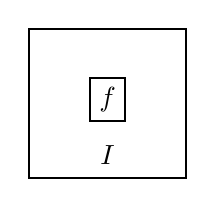
\begin{tikzpicture}[
    scale=1,
    line width=0.8pt,
]
%bounding box
\draw (-1,0) rectangle (1,1.9);

\node[draw, rectangle] (f) at (0,1) {$f$};
\node at (0, 0.3) {$\gr{I}$};
\end{tikzpicture}}
%end polynomial
\end{equation}

\hfill
\begin{tikzcd}
    R^{I} \\
    R^{I}  \otimes_{R^{Ii}} R^{I}  \arrow[u, "m"]
\end{tikzcd}
\hfill
\begin{tikzcd}
    R^{Ii} \\
    R^{I} \arrow[u, "\dd"]
\end{tikzcd}
\hfill 
\begin{tikzcd}
    R^{I} \\
    R^{Ii}  \arrow[u, "\iota"]
\end{tikzcd}
\hfill
\begin{tikzcd}
    R^{I}  \otimes_{R^{Ii}} R^{I}  \\
    R^{I} \arrow[u, "\Delta"]
\end{tikzcd}
\hfill
\begin{tikzcd}[column sep=0em]
     R^I  &f\\
   R^I \arrow[u] &1 \arrow[u, mapsto]
\end{tikzcd}.
\hfill
\vspace{15pt}

\begin{equation}\label{diag generating crossings}
\hfill
{
\begin{tikzpicture}[
    scale=1,
    line width=0.8pt,
    % Updated style to place two arrows on each line
    arrow_style/.style={
        decoration={
            markings,
            mark=at position 0.3 with {\arrow{Stealth[black]}}, % First arrow
            mark=at position 0.8 with {\arrow{Stealth[black]}}  % Second arrow
        },
        postaction={decorate}
    }
]

% Draw the two intersecting lines
\draw[color={rgb,255:red,0; green,0; blue,192}, arrow_style] (1,-1) -- (-1,1);
\draw[red, arrow_style] (-1,-1) -- (1,1);



% Place the labels in the quadrants
\node at (0, 0.7) {$\gr{Ii}$};
\node at (0.8, 0) {$\gr{Iij}$};
\node at (0, -0.7) {$\gr{Ij}$};
\node at (-1, 0) {$\gr{I}$};
\node at (1.7,0) {};
\node at (-1.7,0) {};
%bounding box
\node[draw, inner sep=0pt, fit=(current bounding box)] {};

\comm{%bounding lines on top and bottom
 % 1. Create an invisible node named (bbox) that fits the diagram with padding.
    % Notice there is no 'draw' option here.
    \node (bbox) [fit=(current bounding box), inner sep=0pt] {};

    % 2. Draw lines using the anchors of the invisible (bbox) node.
    \draw[black] (bbox.north west) -- (bbox.north east); % Top line
    \draw[black] (bbox.south west) -- (bbox.south east); % Bottom line
}
\end{tikzpicture}
}
\hspace{100 pt}
{
\begin{tikzpicture}[
    scale=1,
    line width=0.8pt,
    % Updated style to place two arrows on each line
    arrow_style/.style={
        decoration={
            markings,
            mark=at position 0.3 with {\arrow{Stealth[black]}}, % First arrow
            mark=at position 0.8 with {\arrow{Stealth[black]}}  % Second arrow
        },
        postaction={decorate}
    }
]

% Draw the two intersecting lines
\draw[color={rgb,255:red,0; green,0; blue,192}, arrow_style] (-1,1) -- (1,-1);
\draw[red, arrow_style] (1,1) -- (-1,-1);



% Place the labels in the quadrants
\node at (0, -0.7) {$\gr{Ii}$};
\node at (-1, 0) {$\gr{Iij}$};
\node at (0, 0.7) {$\gr{Ij}$};
\node at (1, 0) {$\gr{I}$};
\node at (1.7,0) {};
\node at (-1.7,0) {};

%bounding box
\node[draw, inner sep=0pt, fit=(current bounding box)] {};

\comm{%bounding lines on top and bottom
 % 1. Create an invisible node named (bbox) that fits the diagram with padding.
    % Notice there is no 'draw' option here.
    \node (bbox) [fit=(current bounding box), inner sep=0pt] {};

    % 2. Draw lines using the anchors of the invisible (bbox) node.
    \draw[black] (bbox.north west) -- (bbox.north east); % Top line
    \draw[black] (bbox.south west) -- (bbox.south east); % Bottom line
}
\end{tikzpicture}
}
\hfill \null
\end{equation}

\begin{tikzcd}[column sep=0em]
    R^{I}  \otimes_{R^{Ii}} R^{Ii} \otimes_{R^{Iij}} R^{Iij}  &f\otimes 1 \otimes 1\\
    R^{I}  \otimes_{R^{Ij}} R^{Ij} \otimes_{R^{Iij}} R^{Iij}  \arrow[u] &f \otimes 1 \otimes 1 \arrow[u, mapsto]
\end{tikzcd}
\hfill
\begin{tikzcd}[column sep=0em]
     R^{Iij} \otimes_{R^{Iij}} R^{Ij}  \otimes_{R^{Ij}}R^{I} &1\otimes 1 \otimes f\\
   R^{Iij} \otimes_{R^{Iij}} R^{Ii}  \otimes_{R^{Ii}}R^{I} \arrow[u] &1 \otimes 1 \otimes f \arrow[u, mapsto]
\end{tikzcd}. \vspace{10 pt}


Note that while the upward and downward crossings are degree zero morphisms, the cups, caps and polynomials need not be. The clockwise cup and cap in the diagrams above have positive degree, given by $\ell(Ii)-\ell(I)$, and the counterclockwise cup and cap have negative degree given by $\ell(I)-\ell(Ii)$. The degree of a polynomial $f$ is determined by its degree as an element of $R$.

The first set of relations in $\mathcal{D}(\Gamma)$ are the isotopy relations (for valid region labelings): 

 \begin{equation} \label{isotopy} \igs{1}{isotopy}, \end{equation} 
\begin{equation} \label{crosscyclic} \igs{1}{crosscyclic}, \end{equation}
\begin{equation}\label{crosscyclic2} \igs{1}{crosscyclic2}. \end{equation}

We also want polynomials $f$ to behave as elements of $R$, so we have the following relation in $\DiagSBS(\Gamma)$ (for valid region labels).
\begin{equation} \label{polymult} \igs{1}{polymult} \end{equation}

\begin{defn}\label{defn diagrammatic precategory}
    We define $\DiagSBS^{\pre}$ to be the diagrammatic category with the same generators as that of $\DiagSBS(\Gamma)$, with the isotopy relations in \cref{isotopy}, \cref{crosscyclic} and \cref{crosscyclic2} imposed, along with \cref{polymult}.
\end{defn}

The following are examples of 2-morphisms in $\DiagSBS^{\pre}$ (as well as in $\DiagSBS(\Gamma)$ and $\DiagSBS$, once defined). As in \cref{sec:combo}, we use $\hh{a}$ to denote the maximal finitary subset $S \setminus \set{a}$.
A label $k$ on a strand corresponds to the simple reflection $s_k$.

\[\begin{array}{cccc}
  \isvg{0.15}{cap_ssbim}    &\isvg{0.15}{cup_ssbim} &\isvg{0.15}{eg_mssbim} 
  &\isvg{0.15}{image_of_trivalent_top_section}
\end{array} 
\]
Note that we sometimes omit the strand and region labels, when these are already determined by the other labels. 
We will also simplify diagrams by drawing them up to isotopy. 
We have sideways crossings obtained by rotating the upward or downward crossings (which is well defined after imposing the isotopy relations) as shown below, for any $Iij \in \mc{F}$. 
\begin{equation}
    {
\begin{tikzpicture}[baseline=-0.5ex,
    scale=1,
    line width=0.8pt,
    % Updated style to place two arrows on each line
    arrow_style/.style={
        decoration={
            markings,
            mark=at position 0.3 with {\arrow{Stealth[black]}}, % First arrow
            mark=at position 0.8 with {\arrow{Stealth[black]}}  % Second arrow
        },
        postaction={decorate}
    }
]

% Draw the two intersecting lines
\draw[color={rgb,255:red,0; green,0; blue,192}, arrow_style] (-1,1) -- (1,-1);
\draw[red, arrow_style] (-1,-1) -- (1,1);



% Place the labels in the quadrants
\node at (0, 0.7) {$\gr{I}$};
\node at (0.8, 0) {$\gr{Ii}$};
\node at (0, -0.7) {$\gr{Iij}$};
\node at (-1, 0) {$\gr{Ij}$};
\node at (1.3,0) {};
\node at (-1.3,0) {};
%bounding box
\node[draw, inner sep=0pt, fit=(current bounding box)] {};

\comm{%bounding lines on top and bottom
 % 1. Create an invisible node named (bbox) that fits the diagram with padding.
    \node (bbox) [fit=(current bounding box), inner sep=0pt] {};

    % 2. Draw lines using the anchors of the invisible (bbox) node.
    \draw[black] (bbox.north west) -- (bbox.north east); % Top line
    \draw[black] (bbox.south west) -- (bbox.south east); % Bottom line
}
\end{tikzpicture}
} := 
    {\begin{tikzpicture}[baseline=-0.5ex,
    scale=1,
    line width=0.8pt,
    % Updated style to place two arrows on each line
    arrow_style/.style={
        decoration={
            markings,
            mark=at position 0.3 with {\arrow{Stealth[black]}}, % First arrow
            mark=at position 0.8 with {\arrow{Stealth[black]}}  % Second arrow
        },
        postaction={decorate}
    }
]
\draw[red, arrow_style] (.5,-1) to (-.5,1);
\draw[color={rgb,255:red,0; green,0; blue,192}, arrow_style] (-1.1,1) to[out=-90,in=-135,looseness=2] (0,0) to [out=45,in=90,looseness=2] (1.1,-1);
\node at (0.7,0.7) {$\gr{Ii}$};
\node at (-.7,-.7) {$\gr{Ij}$};
\node at (.5,-.2) {$\gr{Iij}$};
\node at (-.5,.2) {$\gr{I}$};
\node at (1.3,0) {};
\node at (-1.3,0) {};
%bounding box
\node[draw, inner sep=0pt, fit=(current bounding box)] {};
\end{tikzpicture}} 
    =
    {\begin{tikzpicture}[baseline=-0.5ex, 
    scale=1,
    line width=0.8pt,
    % Updated style to place two arrows on each line
    arrow_style/.style={
        decoration={
            markings,
            mark=at position 0.3 with {\arrow{Stealth[black]}}, % First arrow
            mark=at position 0.8 with {\arrow{Stealth[black]}}  % Second arrow
        },
        postaction={decorate}
    }
]
\draw[color={rgb,255:red,0; green,0; blue,192}, arrow_style] (.4,1) to (-.4,-1);
\draw[red, arrow_style] (-1.1,-1) to[out=90,in=135,looseness=2] (0,0) to [out=-45,in=-90,looseness=2] (1.1,1);
\node at (0.7,-.7) {$\gr{Ii}$};
\node at (-.7,.7) {$\gr{Ij}$};
\node at (.5,.3) {$\gr{I}$};
\node at (-.5,-.3) {$\gr{Iij}$};
\node at (1.3,0) {};
\node at (-1.3,0) {};
%bounding box
\node[draw, inner sep=0pt, fit=(current bounding box)] {};
\end{tikzpicture}}.
\end{equation}
\begin{equation}
    {
\begin{tikzpicture}[baseline=-0.5ex,
    scale=1,
    line width=0.8pt,
    % Updated style to place two arrows on each line
    arrow_style/.style={
        decoration={
            markings,
            mark=at position 0.3 with {\arrow{Stealth[black]}}, % First arrow
            mark=at position 0.8 with {\arrow{Stealth[black]}}  % Second arrow
        },
        postaction={decorate}
    }
]

% Draw the two intersecting lines
\draw[color={rgb,255:red,0; green,0; blue,192}, arrow_style] (1,-1) -- (-1,1);
\draw[red, arrow_style] (1,1) -- (-1,-1);



% Place the labels in the quadrants
\node at (0, 0.7) {$\gr{Iij}$};
\node at (0.8, 0) {$\gr{Ij}$};
\node at (0, -0.7) {$\gr{I}$};
\node at (-1, 0) {$\gr{Ii}$};
\node at (1.3,0) {};
\node at (-1.3,0) {};
%bounding box
\node[draw, inner sep=0pt, fit=(current bounding box)] {};

\comm{%bounding lines on top and bottom
 % 1. Create an invisible node named (bbox) that fits the diagram with padding.
    \node (bbox) [fit=(current bounding box), inner sep=0pt] {};

    % 2. Draw lines using the anchors of the invisible (bbox) node.
    \draw[black] (bbox.north west) -- (bbox.north east); % Top line
    \draw[black] (bbox.south west) -- (bbox.south east); % Bottom line
}
\end{tikzpicture}
} := 
    {\begin{tikzpicture}[baseline=-0.5ex,
    scale=1,
    line width=0.8pt,
    % Updated style to place two arrows on each line
    arrow_style/.style={
        decoration={
            markings,
            mark=at position 0.3 with {\arrow{Stealth[black]}}, % First arrow
            mark=at position 0.8 with {\arrow{Stealth[black]}}  % Second arrow
        },
        postaction={decorate}
    }
]
\draw[red, arrow_style] (-.5,1) to (.5,-1);
\draw[color={rgb,255:red,0; green,0; blue,192}, arrow_style] (1.1,-1) to[out=90,in=45,looseness=2] (0,0) to [out=-135,in=-90,looseness=2] (-1.1,1);
\node at (0.7,0.7) {$\gr{Ij}$};
\node at (-.7,-.7) {$\gr{Ii}$};
\node at (.5,-.2) {$\gr{I}$};
\node at (-.5,.2) {$\gr{Iij}$};
\node at (1.3,0) {};
\node at (-1.3,0) {};
%bounding box
\node[draw, inner sep=0pt, fit=(current bounding box)] {};
\end{tikzpicture}} 
    =
    {\begin{tikzpicture}[baseline=-0.5ex, 
    scale=1,
    line width=0.8pt,
    % Updated style to place two arrows on each line
    arrow_style/.style={
        decoration={
            markings,
            mark=at position 0.3 with {\arrow{Stealth[black]}}, % First arrow
            mark=at position 0.8 with {\arrow{Stealth[black]}}  % Second arrow
        },
        postaction={decorate}
    }
]
\draw[color={rgb,255:red,0; green,0; blue,192}, arrow_style] (-.5,-1) to (.5,1);
\draw[red, arrow_style] (1.1,1) to[out=-90,in=-45,looseness=2] (0,0) to [out=135,in=90,looseness=2] (-1.1,-1);
\node at (0.7,-.7) {$\gr{Ij}$};
\node at (-.7,.7) {$\gr{Ii}$};
\node at (.5,.3) {$\gr{Iij}$};
\node at (-.5,-.3) {$\gr{I}$};
\node at (1.3,0) {};
\node at (-1.3,0) {};
%bounding box
\node[draw, inner sep=0pt, fit=(current bounding box)] {};
\end{tikzpicture}}.
\end{equation}

Unlike the upward and downward crossings, these are not always of degree 0. The degree of the sidewards crossings given above are $\ell(Iij)+\ell(I)-\ell(Ii)-\ell(Ij)$. A mnemonic for the degree of the sideways crossings is ``big + small - middle - middle". We will henceforth use sidewards crossings in our diagrams and draw diagrams up to isotopy without explicit mention.

% \PT{Should I just add a sidward crossing earlier explicitly and write down its degree?} \BE{My mnemonic for the degree is big + small - middle - middle. The reason for doing this would be to justify, later, that the image of GS lives in degree zero. Worth having as a lemma?}\PT{Added below. Check.} \BE{No... this lemma here you can cite instead... the lemma the verbal argument below that the degree of the image of the trivalent vertex is zero can be made a short lemma, but stated cleanly enough that you can cite it later.}


For example, the diagram in the RHS of the equation below will appear multiple times in later sections.
\begin{equation}\label{eq trivalent split}\isvg{0.15}{trivalent_split}= \isvg{0.2}{image_of_down_trivalent}\end{equation}
\begin{lemma}\label{lemma image of trivalent has degree 0}
    The 2-morphism in \cref{eq trivalent split} is of degree 0.
\end{lemma}
\begin{proof}
The rotation operator $\sigma$ (\cref{defn-rotation operator}) preserves lengths of parabolic subgroups, hence without loss of generality, we may assume $a=0$. 
The sidewards crossing in \cref{eq trivalent split} then has degree $\ell(\hh{l})+\ell(\hh{0,l,k+l})-\ell(\hh{0, l})-\ell(\hh{l, k+l})$ and the counter-clockwise cup has degree $\ell(\hh{0, l, k+l})-\ell(\hh{0, k+l})$. Note that the parabolic subgroups $W_{\hh{0,l,k+l}}, W_{\hh{0, l}}$ etc. are just a product of symmetric groups $S_l\times S_k \times S_{n-k-l}, S_l \times S_{n-l}$ etc., so that the net degree is 
\begin{align*}
    &\ell(\hh{l})+2\ell(\hh{0,l,k+l})-\ell(\hh{0, l})-\ell(\hh{l, k+l})-\ell(\hh{0, k+l})\\
    &= \binom{n}{2} + 2\left(\binom{l}{2}+\binom{k}{2}+\binom{n-k-l}{2}\right) - \left(\binom{l}{2}+\binom{n-l}{2}\right)\\
    &\qquad-\left(\binom{k}{2}+\binom{n-k}{2}\right)-\left(\binom{n-k-l}{2}+\binom{k+l}{2}\right)
    \\
    &=
    \binom{n}{2}+\binom{l}{2}+\binom{k}{2}+\binom{n-k-l}{2}-\binom{n-l}{2}-\binom{n-k}{2}-\binom{k+l}{2}=0. \qedhere
\end{align*}
\end{proof}

We now continue discussing the relations in $\DiagSBS(\Gamma)$.
All future relations hold when rotated or with the colors switched, but not with the orientations reversed. 
%We have the relations which hold for any Frobenius extension $\iota : A \subset B$. 

Consider $I, Ii \in \mc{F}$. 
We have the following relations associated to the Frobenius extension $(R^{Ii}\hookrightarrow R^I, \dd=\dd^I_{Ii})$.

\begin{equation} \label{polyslide} \igs{1}{polyslide} \end{equation}
\begin{equation} \label{cccirc} \igs{1}{cccirc} \end{equation}
\begin{equation} \label{ccwcirc} \igs{1}{ccwcirc} \end{equation}
\begin{equation} \label{Bsplitting} \igs{1}{Bsplitting} \end{equation}
In \cref{Bsplitting}, we use the Sweedler notation from \cref{subsubsec-notation in further calculations.}
%: having a $\Delta^B_{A}{}_{(1)}$ and $\Delta^B_{A}{}_{(2)}$ in the same expression indicates a sum over a dual basis $\set{x_i}, \set{y_i}$ for the extension $A \subset B$, i.e., we substitute $x_i$ for $\Delta^B_{A}{}_{(1)}$ and $y_i$ for $\Delta^B_{A}{}_{(2)}$ and take a sum over $i$.

Now consider $I, Ii, Iij \in \mc{F}$. 
We then have the following \emph{Reidemeister II relations}.


\begin{equation} \label{R2oriented} \igs{0.8}{R2oriented} \end{equation}
\begin{equation} \label{R2unoriented1} \igs{0.8}{R2unoriented1} \end{equation}
\begin{equation} \label{R2unoriented2} \igs{0.8}{R2unoriented2} .\end{equation}
The polynomial in the box in \cref{R2unoriented2} is  $\mu_{Iij}^{Ii, Ij}$ (see \cref{subsubsec-notation in further calculations.}).
The RHS of \cref{R2unoriented1} may be written in several equivalent ways using the following identity specialized at $f=1$:
\begin{align}\label{eq R2 unoriented equivalent formulas}
\notag \Delta^{Ii}_{Iij, (1)} \otimes  \dd^I_{Ij}(f\Delta^{Ii}_{Iij, (2)})= \dd^I_{Ii}(f\Delta^I_{Iij,(1)})\otimes \dd^I_{Ij}(\Delta^I_{Iij,(2)})&=\dd^I_{Ii}(\Delta^I_{Iij,(1)})\otimes \dd^I_{Ij}(f\Delta^I_{Iij,(2)})\\
= \dd^I_{Ii}(f\Delta^{Ij}_{Iij,(1)})\otimes \Delta^{Ij}_{Iij, (2)} & \qquad\text{for $f \in R^I$}.
\end{align}
The equation \eqref{eq R2 unoriented equivalent formulas} is a consequence of \cite[(2.7), Section 2.2]{EWSFrob}.



We mention a special instance where \cref{R2unoriented1}, \cref{R2unoriented2} become easier.
When $i$ and $j$ are in different connected components of $Iij \in \mc{F}$, we have that $\Phi_{Iij}^+ \setminus \Phi_{Ii}^+=\Phi_{Ij}^+ \setminus \Phi_I^+$, so that $\mu_{Iij}^{Ii, Ij}=\frac{\mu_{Iij}^{Ii}}{\mu_{Ij}^I}=1.$
We also have that $\dd^{I}_{I\sqcup \set{j}}=\dd^{I\sqcup \set{i}}_{I\sqcup \set{i,j}}$ in this case (for example, by using \cref{corollary-normalization}), so that all but one term on the RHS of \cref{R2unoriented1} vanish.
Hence both the LHS and RHS of the relations \cref{R2unoriented1}\;\;, \cref{R2unoriented2} are degree zero maps in this case, and we have the following \emph{distant Reidemeister II} relations (shortened as \emph{distant RII}).

\begin{align}\label{R2 distant}
 \isvg{0.15}{R2_easy_distant_ssbim_LHS}= \isvg{0.15}{R2_easy_distant_ssbim_RHS}, \qquad\isvg{0.15}{R2_distant_ssbim_LHS}= \isvg{0.15}{R2_distant_ssbim_RHS}.   
\end{align}


Now consider $I \in F$ and $i,j,k \in \Gamma$ such that $Iijk \in \mc{F}$. 
We have the following \emph{Reidemeister III relation}.

\begin{equation} \label{R3oriented} \igs{0.9}{R3oriented} .\end{equation}

%We note here that all the above relations hold in $\mc{C}(\Gamma)$ via $\Phi$ for any hypercube $\Gamma.$

%The following additional relations hold when the cube also satisfies $\star$ (\cref{defn-condition star}), has no $\mu$-zero divisors (\cref{defn- no mu zero deivisors}), and satisfies condition R3 (\cref{defn-condition R3}).
%We have an additional Reidemeister II relation
% \begin{equation} \label{R2unoriented2} \igs{0.8}{R2unoriented2} .\end{equation}
% The polynomial in the box is \BE{you already have this you can call upon it.}
% $\dd_{Ii}^I(\Delta^{Ij}_{Iij,(1)})\Delta^{Ij}_{Iij,(2)}$, which may also be written as $\dd_{Ij}^I(\Delta^{Ii}_{Iij,(1)})\Delta^{Ii}_{Iij,(2)}$, or as
% $\frac{\mu_{Iij}\mu_I}{\mu_{Ii} \mu_{Ij}}$. Consequently, $\frac{\mu_{Iij}\mu_I}{\mu_{Ii} \mu_{Ij}}$ is a genuine polynomial, not just an element of the
% localization.

We also have the \emph{hard Reidemeister III relation}:
\begin{equation} \label{R3unoriented}
  \igs{0.9}{R3unoriented}. \end{equation} The polynomial in the
box is $\frac{\mu_{Iijk} \mu_{Ii} \mu_{Ij}\mu_{Ik}}{\mu_{Iij} \mu_{Iik} 
\mu_{Ijk} \mu_I}$, which is a genuine polynomial by assumption R3 (\cref{defn-condition R3}).

We mention a special case of \cref{R3unoriented}, which will be used in \cref{subsec- I=H}. 
When $i,j,k$ are not in the same component of $Iijk$, we have the following relation which we refer to as the \emph{distant Reidemeister III} relation, usually shortened to \emph{distant RIII}.
\begin{align} \label{distantR3}
\isvg{0.15}{R3_distant_ssbim_LHS}=\isvg{0.15}{R3_distant_ssbim_RHS}.
\end{align}
We leave it as an exercise to the reader to check that the polynomial in the box in the RHS of \cref{R3unoriented} is 1 in this case, so that \cref{distantR3} is indeed just a special case of \cref{R3unoriented}.

% Note that we define $D(\Gamma)$ only for $\Gamma$ satisying the extra conditions, so that this extra set of relations in $\eqref{R3unoriented}$ hold in $\mc{C}(\Gamma)$ via $\Phi$.

%==========================================================================
%\subsection{Diagrammatic Singular Bott-Samelson bimodules}\label{subsec-diagrammatic singular bott-samelson bimodules}
%==========================================================================

% Now we describe diagrammatics for $\SBSBim$.
% Let $\pdSBSBim$ denote the diagrammatic category (from \cref{subsec-diagrammatics for frob hypercube}) associated to the Frobenius hypercube from the deformed affine realization (\cref{defn deformed affine frobenius realization}). 
% %Let $\pdmSBSBim$ denote the full sub-2-category of $\pdSBSBim$ with objects given by maximal finitary subsets of $S$. 
% There is a canonical functor $\tilde{\Phi}: \pdSBSBim \rightarrow \SBSBim$ (as described in \cref{subsec-diagrammatics for frob hypercube}).
% %which restricts to a functor which we again denote by $\Phi$, so that $\Phi: \pdmSBSBim \rightarrow \mSBSBim$.
% Note that we include the additional relations \cref{R2unoriented2}, \cref{R3unoriented} in $\pdSBSBim$ by \cref{lemma deformed affine frobenius satisfies extra conditions}.


The 2-functor $\Phi: \DiagSBS(\Gamma)$ has a kernel, and we define $\dSBSBim$ to be the 2-category obtained by killing the kernel, so that $\Phi$ factors through a faithful functor $\DiagSBS \rightarrow \SBSBim$, which we again denote by $\Phi$.
%We further restrict this to the quotient $\dmSBSBim$ of $\pdmSBSBim$ to get $\tilde{\Phi}:\dmSBSBim \rightarrow \mSBSBim$.

%\BE{Maybe better to say: there is a kernel. define blah to be the quotient by the kernel. some elements of the kernel are known, but it is not known whether there are enough relations.}
\PTv2{Still retaining this comment in case we want to talk a bit more about the kernel.}


Recall that $\sigma$ and $\tau$ denoted automorphisms of the affine Dynkin diagram, which extended to automorphisms of $\Lambda_\zeta$ and $R$. 
We use these automorphisms to define certain symmetries of $\DiagSBS^{\pre}$ and $\SBSBim$, which descend also to $\DiagSBS(\Gamma)$ and $\DiagSBS$.

\begin{defn} \label{defn:symmetries of diagsbs} 
%We define $2$-functors $\sigma, \rotation, \Upsilon_S \colon \DiagSBS \to \DiagSBS$, the basic symmetries of this category. Note that $\sigma$ and $\tau$ (also) denote automorphisms of the affine Dynkin diagram.

% On objects/region labels $\sigma$ sends $I \mapsto \sigma(I)$, e.g. it sends $\hh{a} \mapsto \hh{a+1}$. This necessarily changes the labeling on edges as well, by applying $\sigma$ to the set of simple reflections. Aside from relabling, diagrams remain unchanged. This is a monoidal, covariant equivalence.

% On objects $\rotation$ sends $I \mapsto I$, and it rotates all diagrams by 180 degrees. This is an antimonoidal, contravariant equivalence.

% On objects $\Upsilon_S$ sends $I \mapsto \tau(I)$, e.g. it sends $\hh{a} \mapsto \hh{-a}$. This necessarily also acts on the edge labeling by $\tau$. It flips each diagram vertically (i.e. reflecting across a horizontal axis), and then reverses the orientation. This is a monoidal, contravariant equivalence.


We define 2-endofunctors $\sigma, \rotation, \Upsilon_S$ on $\DiagSBS^{\pre}$ and $\SBSBim$ as follows. 

On objects/region labels $\sigma$ sends $I \mapsto \sigma(I)$, e.g. it sends $\hh{a} \mapsto \hh{a+1}$. On $\DiagSBS$, this necessarily changes the labeling on edges by applying $\sigma$ to the set of simple reflections, and changes floating polynomials by applying $\sigma$ on polynomials. 
Aside from relabeling and changing polynomials, diagrams remain unchanged. 
On $\SBSBim$, the action of $\sigma$ on $\Hom(I,J)$ is obtained from the equivalence of graded $(R^I,R^J)$-bimodule categories induced by the isomorphism of graded algebras $R^I\otimes R^J\xrightarrow[\sigma \otimes \sigma]{\sim}R^{\sigma(I)}\otimes R^{\sigma(J)}$.
This is a monoidal, covariant equivalence.

On objects $\rotation$ sends $I \mapsto I$. On $\DiagSBS^{\pre}$, it rotates all diagrams by 180 degrees and leaves floating polynomials unchanged. Note that this 2-functor coincides with combining a horizontal flip and a vertical flip in either order.
On $\SBSBim$, $\rotation$ is obtained from adjunctions, but may also be thought of as a composition of natural symmetries corresponding to horizontal and vertical flips; see \cref{subsec reversal duality and phi} (in particular \cref{def rotation by 180 degrees}, \cref{corollary phi intertwines rotation} and \cref{rmk rotation and flips and adjunctions}) for the details. 
This is an antimonoidal, contravariant equivalence.

On objects $\Upsilon_S$ sends $I \mapsto \tau(I)$, e.g. it sends $\hh{a} \mapsto \hh{-a}$. This necessarily also acts on the edge labeling and on floating polynomials by $\tau$. It flips each diagram vertically (i.e. reflecting across a horizontal axis), reverses arrows to be consistent with region labels, and acts on any floating polynomials by $\tau$. 
On $\SBSBim$, $\Upsilon_S$ acts on 1-morphism categories via 
$$\Hom(I,J)^{op} \xrightarrow[D]{} \Hom(I,J) \xrightarrow[\tau_{\#}]{} Hom(\tau(I),\tau(J)),$$ where
$$D: \Hom(I,J)^{\op}\xrightarrow{\sim} \Hom(I,J): B \mapsto \Hom^\bullet_{R^J}(B, R^J)(2\ell(I)-2\ell(J)) $$ 
denotes the duality functor (see \cref{def duality symmetry D algebraic}),
and 
$$\tau_{\#}:\Hom(I,J) \xrightarrow{\sim} Hom(\tau(I),\tau(J))$$
is induced by the isomorphism of graded algebras $R^I\otimes R^J \xrightarrow[\tau \otimes \tau]{\sim}R^{\tau(I)}\otimes R^{\tau(J)}.$ 
This is a monoidal, contravariant equivalence. 

% \BE{instead of leave it to the reader, refer to appendix (you leave it to the reader there...)}\PT{Well, not the one including $\sigma$ and $\tau$, which is easy. Appendix only describes duality, reversal and rotation, the rest are still exercises. And I really don't want to add $\tau$ and $\sigma$  stuff to the appendix...(Tbh I'm tired of writing!). We're already doing enough community service in this paper.} %We leave it to the reader to show that t
The 2-functor $\Phi: \DiagSBS^{\pre} \to \SBSBim$ intertwines the 2-equivalences $\sigma, \rotation, \Upsilon_S$, so that these 2-equivalences descend to $\DiagSBS(\Gamma)$ and $\DiagSBS$. 
Note here that ``intertwine" is not just a condition, but the data of certain natural isomorphisms (cf. \cref{thm phi commutes with dual and rev}, \cref{corollary phi intertwines rotation}).
We denote these 2-functors on $\mc{D}(\Gamma), \DiagSBS$ again by $\sigma, \rotation, \Upsilon_S$.
\end{defn}


\begin{remark} Unlike the category of webs, it would be absurd in $\DiagSBS$ to reverse the orientations of the strands without flipping, or vice versa. \end{remark}

%==========================================================================
\subsection{The functor \texorpdfstring{$\GS_{\zeta}$}{GS\_zeta}}\label{subsec the functor}
%==========================================================================


Define $\cwebs$ and $\dmSBSBim$ over the base ring $A=A_{\Z}\otimes_{\Z} \Q$,  
where $A_{\Z}$ is as in \cref{eq coefficient ring with q and zeta}, i.e.,
$A_{\Z}= \begin{cases}
\Z[q^{\pm 1}, \zeta^{\pm 1}]/(q^{-2}-\zeta^n) &\text{if $n$ odd;}\\
\Z[q^{\pm 1}, \zeta^{\pm 1}]/(q^{-1}-\zeta^{n/2}) &\text{if $n$ even.}
    \end{cases}$
    
\begin{defn}\label{defn dQGS functor}
Let $(\lambda, \nu)$ denote a collection of scalars $\lambda_k, \nu_k \in A^\times$ for various $1 \le k < n$, and scalars $\lambda_{k,l}, \nu_{k,l} \in A^{\times}$ for various $1 \le k,l < n$ with $k+l < n$. Attempt to define an $A$-linear $2$-functor $\GS_{\zeta} = \GS_{\zeta}(\lambda, \nu): \cwebs \rightarrow \dmSBSBim$ as follows. 

On objects, we have the bijection 
\begin{equation}\label{eq dQGS on objects}a \mapsto \hh{a}\end{equation}
for any 
$1\leq a \leq n$, where $\hh{a}$ is the maximal finitary subset $S\setminus \set{a} \subset S$.

On generating 1-morphisms, we have
\begin{align}\label{eq dQGS on 1-morphisms}
\notag \gr{a+k}\uparrow^{\blk{k}} \gr{a} \mapsto \dgr{a+k} \downarrow \dgr{a, a+k}\uparrow \dgr{a}    \\
\gr{a-k}\downarrow^{\blk{k}} \gr{a} \mapsto \dgr{a-k} \downarrow \dgr{a, a-k}\uparrow \dgr{a}    
\end{align}

On generating two morphisms, we have:
\begin{align}\label{diag-dQGS on 2-morphisms}
\notag&\isvg{0.15}{cap_webs_c} \mapstosize{2} \isvg{0.15}{cap_ssbim_c} (-1)^{k(n-k)}\hspace{10 pt}
&&\isvg{0.15}{cap_webs_cc} \mapstosize{2} \isvg{0.15}{cap_ssbim_cc} \vspace{5 pt}\\
\notag&\isvg{0.15}{cup_webs_c} \mapstosize{2}  \isvg{0.15}{cup_ssbim_c}
&&\isvg{0.15}{cup_webs_cc} \mapstosize{2} \isvg{0.15}{cup_ssbim_cc} (-1)^{k(n-k)}\vspace{5pt}\\
\notag&\isvg{0.15}{tag_left_c}  \mapstosize{2} \isvg{0.15}{image_of_tag_c}\; \lambda_k 
&&\isvg{0.15}{tag_left_d} \mapstosize{2} \isvg{0.15}{image_of_tag_d} \;\nu_k\vspace{5pt}\\
&\isvg{0.15}{trivalent_vertex_up}    \mapstosize{2} \isvg{0.15}{image_of_up_trivalent}\; \lambda_{k,l} 
&&\isvg{0.15}{trivalent_vertex_down}  \mapstosize{2} \isvg{0.15}{image_of_down_trivalent}\; \nu_{k,l}.
\end{align}
\end{defn}

\begin{defn}\label{defn convention for coefficients of trivalent with labels n} We introduce the following convention. Let $\lambda_{k,n-k}:=\lambda_k$ and $\nu_{k,n-k}:=(-1)^{k(n-k)}\nu_{n-k}$. \end{defn}

\begin{remark}\label{rmk compatibility of convention for lambdanu-k,(n-k) as lambdanu-k}
This convention is compatible with the convention that a tag can be thought of as a trivalent vertex with one strand (replacing the tag) having label $n$. 
\end{remark}

\begin{theorem} \label{thm dQGS functor}
The $2$-functor $\GS_{\zeta}(\lambda, \nu)$ is well-defined if and only if the scalars $(\lambda, \nu)$ satisfy the relations below for all $k, l, m$. By convention, if the indices are not within the range $\{1, \ldots, n-1\}$ then omit the relation. 
\begin{subequations} \label{scalarconditions}
\begin{gather}
   \lambda_k= \lambda_{n-k}, \quad \nu_k=\nu_{n-k} \label{cond-tag switching}\\ 
    \lambda_k= \nu_k^{-1}\label{cond-tag cancellation}\\ 
    \lambda_{k,l}\lambda_{k+l,m}= \lambda_{k,l+m}\lambda_{l,m}, \quad \nu_{k, l+m}\;\nu_{l,m}=\nu_{k+l,m}\nu_{k,l} \label{cond-I=H relation}\\  
    \lambda_{k-1,1}\nu_{k-1,1}= (-1)^{k-1}\zeta^{\frac{k(k-1)}{2}}q^{k-1}. \label{cond-bigon killing}
\end{gather}
\end{subequations}
\end{theorem}

\begin{proof}
In \cref{sec well-defined-ness of the functor}, we show that the conditions \cref{cond-tag switching}-\cref{cond-bigon killing} are the only constraints implied by the web relations in \cref{fig:webrel} (along with their mirror images and arrow reversals.)
\end{proof}

\begin{example} \label{goodchoiceoflambdanu}
One can check that 
\begin{equation} \lambda_{k,l}:=\zeta^{\frac{kl(k+l)}{2}}(-q)^{kl}, \quad \nu_{k,l}=1, \quad \lambda_{k}=\nu_k = (-1)^{k(n-k)} \end{equation} is a solution to the above equations.
Note that this example is compatible with the convention in \cref{defn convention for coefficients of trivalent with labels n}.
\end{example}

Having postponed this proof to the next chapter, we spend the remainder of this chapter discussing the scalars $(\lambda, \nu)$.




% then the images of trivalent vertices with $k+l=n$ is coincides with the images of cups or caps with a coefficient $\lambda_{k,n-k}$ or $\nu_{k,n-k}$. 


\begin{lemma}\label{lemma coefficient symmetry}
   Conditions \cref{cond-tag switching}-\cref{cond-bigon killing} imply that \begin{align*}
       \lambda_{k,l}=\lambda_{l,k}, \quad \quad \nu_{k,l}=\nu_{l,k}
   \end{align*}
   for any $1\leq k,l \leq n-1$ such that $k+l \leq n$.
\end{lemma}
\begin{proof}
    Condition \cref{cond-tag switching} implies that the lemma holds when $k+l=n$, so we  need only prove the lemma for $k+l \leq n-1$.

    First we show that $\lambda_{1,m}=\lambda_{m,1}$ for any $1 \leq m < n-1$ using induction on $m$. 
    The base case $m=1$ is trivial, so suppose now that $m>1$. 
    From condition \cref{cond-I=H relation}, we have that
    $$\lambda_{1,m-1}\lambda_{m,1}=\lambda_{1,m}\lambda_{m-1,1}.$$ 
    But $\lambda_{1,m-1}=\lambda_{m-1,1}$ by induction hypothesis, so $\lambda_{m,1}=\lambda_{1,m}$ as desired.
    
    Now we discuss the general case. 
    Condition \cref{cond-I=H relation} implies that
    for any $1\leq k \leq n-1$, $1<l \leq n-1$ such that $k+l \leq n-1$, we have $\lambda_{k,l-1}\lambda_{k+l-1,1}=\lambda_{k,l}\lambda_{l-1,1}$, so that $\dfrac{\lambda_{k,l+1}}{\lambda_{k,l}}=\dfrac{\lambda_{k+l,1}}{\lambda_{l,1}}$.
    We then iteratively have that
    \begin{align*}
     \frac{\lambda_{k,l}}{\lambda_{k,1}}= \frac{\lambda_{k+1,1}}{\lambda_{1,1}}\frac{\lambda_{k+2,1}}{\lambda_{2,1}}\ldots \frac{\lambda_{k+l-1,1}}{\lambda_{l-1,1}}
    \end{align*}
    so that 
    \begin{align}
    \lambda_{k,l}=\lambda_{k,1}\frac{\lambda_{k+1,1}}{\lambda_{1,1}}\frac{\lambda_{k+2,1}}{\lambda_{2,1}}\ldots \frac{\lambda_{k+l-1,1}}{\lambda_{l-1,1}}.\label{eq 1 lemma coefficient symmetry}
    \end{align}
    Similarly, using that
    $\lambda_{1,l-1}\lambda_{l,k}=\lambda_{1,k+l-1}\lambda_{l-1,k}$, we have that 
    \begin{align}
      \lambda_{l,k} =\lambda_{1,k}\frac{\lambda_{1,k+1}}{\lambda_{1,1}}\frac{\lambda_{1,k+2}}{\lambda_{1,2}}\ldots \frac{\lambda_{1,k+l-1}}{\lambda_{1,l-1}} \label{eq 2 lemma coefficient symmetry}.
    \end{align}
    The RHS of \cref{eq 1 lemma coefficient symmetry} and \cref{eq 2 lemma coefficient symmetry} are equal by the special case of the lemma when one of the indices is 1, so we have that $\lambda_{k,l}=\lambda_{l,k}$ as desired.
\end{proof}

\begin{lemma}\label{lemma symmetry of GS-zeta}
The 2-functor $\GS_\zeta$ intertwines the symmetries $\sigma$ and $\Upsilon_W$ of $\cwebs$ with the symmetries $\sigma$ and $\Upsilon_S$ of $\DiagSBS$ respectively. It intertwines $\rotation$ with $\rotation$, up to sign. More precisely, we have 
\begin{equation}\label{eq GS-zeta intertwines symmetries}
\GS_\zeta \circ \sigma=\sigma \circ \GS_\zeta, \quad \GS_\zeta \circ \Upsilon_W=\Upsilon_S \circ \GS_\zeta,  \quad \rotation \circ \GS_{\zeta} = \GS_{\zeta} \circ \rotation \circ \scalewebs,
\end{equation} 
where $\scalewebs$ is the object-fixing automorphism of $\cwebs$ that multiplies each web by $(-1)^{k(n-k)}$ for each upward-oriented $k$ in the source or target (downward-oriented strands have no effect)\footnote{For example, $\scalewebs$ multiplies all the generators in Definition 5.4 by $(-1)^{k(n-k)}$, except for the trivalent vertices which it multiplies by $(-1)^{k(n-k) + l(n-l) + (k+l)(n-k-l)} = 1$. The 2-functor $\scalewebs$ is isomorphic to the identity 2-functor; the natural isomorphism between them is multiplication by the appropriate sign on each object (a factor of $(-1)^{k(n-k)}$ for each upward-oriented $k$-labeled strand). Hence $\rotation\circ\GS_\zeta\cong\GS_\zeta \circ \rotation$, so that $\GS_\zeta$ also weakly intertwines with rotation.}.
\end{lemma}

\begin{proof}
    It suffices to check this on the generating 2-morphisms, under the assumptions in \cref{thm dQGS functor}. This check is an easy exercise and is left to the reader, where \cref{lemma coefficient symmetry} may be used to check the intertwining of $\Upsilon_W$ and $\Upsilon_S$.

    % \PT{Alternative proof if we add what I suggested to the statement of the lemma:}
    % That the equalities in \cref{eq GS-zeta intertwines symmetries} hold, is a direct check on the generating 2-morphisms (where \cref{lemma coefficient symmetry} may be used in the checks involving $\Upsilon_W$ and $\Upsilon_S$).
    % That the prescribed 2-morphisms specify an intertwining structure in the case of $\rotation$ can also be reduced to a check on the generating 2-morphisms, since the specified 2-morphisms are already compatible with 1-morphism composition. (The specified 2-morphisms are just identity 2-morphisms with a sign given a product of the factors $(-1)^{k(n-k)}$  corresponding to each upward arrow labeled $k$ in the given 1-morphism in $\cwebs$). We leave these checks to the reader.
\end{proof}

\begin{remark} The symmetries are intertwined not because of any application of relations, but already at the level of the diagrams themselves. 
To elaborate, one could define a ``free pivotal'' version $\Webs^{\Om, \pre}$ of webs which have isotopy relations but no other relations. 
One could define a version $\widetilde{\GS}_{\zeta}: \Webs^{\Om, \pre} \rightarrow \DiagSBS^{\pre}$ of $\GS_{\zeta}$; this functor would still involve scalars $\lambda$ and $\nu$ satisfying \eqref{scalarconditions}. 
% To elaborate, one could define ``free pivotal'' versions of both webs and Soergel diagrammatics, which have isotopy relations but no other relations. \BE{incorporate earlier def of Dpre, or delete earlier def of Dpre} 
% One could define a version $\widetilde{\GS}_{\zeta}$ of $\GS_{\zeta}$ between these free categories; this functor would still involve scalars $\lambda$ and $\nu$ satisfying \eqref{scalarconditions}. 
Then \cref{lemma symmetry of GS-zeta} applies to $\widetilde{\GS}_{\zeta}$ as well, and descends to the corresponding result for $\GS_{\zeta}$. We mention this point because, as is common in the field, we use symmetries to check the well-definedness of $\GS_{\zeta}$ itself. We check certain relations, and then claim others hold by applying $\sigma$ or $\Upsilon$ or rotation. There is no fallacy in applying these symmetries before knowing of the existence of the $2$-functor, because we are really applying the symmetries to $\widetilde{\GS}_{\zeta}$. \end{remark}

\begin{remark} One might hope for a symmetry of $\DiagSBS$ corresponding to the arrow-reversing symmetry $\reversal$ of $\cwebs$. It would act on objects and $1$-morphisms by $\tau$. As evidenced by \eqref{diag-dQGS on 2-morphisms}, the inward-pointing tag (with label $k$ on bottom) is sent to an identity map times $\lambda_k$, and any autoequivalence of $\DiagSBS$ sends identity maps to identity maps. Applying $\reversal$ we obtain the outward-pointing tag, which goes to the corresponding identity map times $\nu_k$. So an intertwining symmetry of $\DiagSBS$ is only possible if $\lambda_k = \nu_k$ for all $k$.  Since $\lambda_k = \nu_k^{-1}$, we have $\lambda_k = \nu_k = \pm 1$. This constraint holds for \cref{goodchoiceoflambdanu}.

However, unlike all the other symmetries, this autoequivalence of $\DiagSBS$ would need to rescale diagrams (rather than merely manipulating them). As evidenced by \eqref{diag-dQGS on 2-morphisms}, a sign $(-1)^{k(n-k)}$ appears in the comparison of the different orientations of a $k$-labeled cap or cup. Worse still, $\lambda_{k,l}$ and $\nu_{k,l}$ are swapped in the comparison for trivalent vertices, and for \cref{goodchoiceoflambdanu} this would entail rescaling some diagrams with both signs and powers of $\zeta$. It is possible that such a symmetry exists.

% ... \BE{worth trying for an hour. Just rescale cups and caps, not up-up crossings. The sideways crossings thereby get rescaled. Powers of $\zeta$ cancel out in cups and caps but not in sideways crossings because of different region labels, somehow.}
\PTv2{I did try for more than an hour, but couldn't figure it out. Let's not add it in v1?}
\end{remark}

% has the following additional properties.
% \begin{enumerate}  
%     \item $\GS_\zeta$ preserves symmetry under relabeling regions by the operator $\sigma$ (on both $\cwebs$ and $\dmSBSBim$). We refer to this as \emph{color symmetry}.\PT{Is this clear enough?} \BE{I don't like the focus on region labels... there's also polynomials... One should probably define the symmetries earlier for each category individually in their own chapters.}
%     \item $\GS_\zeta$ intertwines rotation by $180^\circ$ in $\cwebs$ with that in $\dmSBSBim$.
%     \item Let $\Upsilon_{W}$ denote the operation on $\cwebs$ where we do a vertical flip (i.e., reflection across a horizontal axis) followed by region relabeling by $\tau$ (so that $\gr{a}$ becomes $\gr{-a}$ etc.).
%     Let $\Upsilon_S$ denote the operation on $\dmSBSBim$ where we do a vertical flip, reverse orientations and relabel regions by $\tau$.
%     Then $\GS_\zeta$ intertwines $\Upsilon_W$ with $\Upsilon_S$. 
% \end{enumerate}
% \end{lemma}
% \begin{proof}
%     It suffices to check this on the generating 2-morphisms, under the assumptions in \cref{thm dQGS functor}. This check is an easy exercise and is left to the reader, where \cref{lemma coefficient symmetry} may be used for (3).
% \end{proof}





% \PT{It may be worthwile to separate out color symmetry from the rest, since it doesn't require any conditions in \cref{thm dQGS functor}, but is rather built into \cref{defn dQGS functor}.} \BE{It's worth it only if you define the symmetries on the pre-categories (before imposing relations), so that you can use it in checking relations carefully.}

% \PT{Below, I'm in the process of adding extra symmetry discussions. Some of them is not preserved by $\GS_\zeta$ and maybe we should avoid this altogether.}
% We now discuss additional symmetries of $\cwebs$ and $\dmSBSBim$ and describe how $\GS_\zeta$ interacts with them. We may do the following operations on diagrams (some of these are contravariant at the 1-morphism and/or at the 2-morphism level):
% \PT{Starting this off in a rough manner. Will clean up.}
% \begin{itemize}
%     \item Relabeling regions using the rotation operator $\sigma.$ (Compatible with $\GS_\zeta$.)
%     \item Rotating diagrams by $180^{\circ}$ (using suitable cups and caps on bottom and top). (Compatible with $\GS_\zeta$.)
%     \item Horizontal flip (reflecting across a vertical axis) and reversing arrows. (Not compatible with $\GS_\zeta$: preserves cups and caps, but interchanges $\lambda_{k,l}, \nu_{k,l}$ for all trivalent including tags, following convention in \cref{defn convention for coefficients of trivalent with labels n}.)
%     \item Vertical flip (reflecting across a horizontal axis) and reversing arrows.
%     \item Reversing arrows and relabeling regions using $\tau$ in $\cwebs$, just relabeling regions using $\tau$ in $\dmSBSBim$.
%     \item Combining any of the above. For example, $\Upsilon_W$ and $\Upsilon_S$ may be seen as a combination of the previous two operations.
% \end{itemize}

\subsection{Fullness and Faithfulness}\label{subsec fullness and faithfulness}
We now work over the fraction field of the base ring $A$ in \cref{subsec the functor}. The fraction field is a finite extension of $\Q(q)$ which we denote $\Q(q,\zeta)$.
Throughout this section, we use $\GS_\zeta$ to refer to the 2-functor $\GS_\zeta(\lambda, \nu)$ in \cref{subsec the functor} for any valid choice of coefficients (see \cref{thm dQGS functor}), and reuse the same notation for the functor (as well as the underlying categories) obtained after extending scalars along the localization map $A \hookrightarrow \Q(q,\zeta)$.

Recall from \cref{subsec-colored sln webs} that we have a factorization $\qFund \xrightarrow{\sim} \cwebs \rightarrow \qRep$ of the canonical inclusion of $\qFund$ into $\qRep$, and that the Karoubi envelope of $\qFund$ coincides with $\qRep$.
The 2-functor $\GS_\zeta: \cwebs \rightarrow \DiagSBS \hookrightarrow \SBSBim$ factors through $m\SBSBim$. We denote the induced map $\cwebs \rightarrow m\SBSBim$ again by $\GS_\zeta$.
Recall from \cref{subsec reverse bott-samelsons} that the Karoubi envelope of (the graded, additive completion of) $m\SBSBim$ coincides with the full sub-category $m\SSBim$ of $\SSBim$.
The 2-functor 
$$\qFund \xrightarrow{\sim} \cwebs \xrightarrow{\GS_\zeta} m\SBSBim$$
then canonically extends to the respective Karoubi envelopes, and we obtain an additive 2-functor $\QGS: \qRep \rightarrow m\SSBim$. 



\begin{lemma}\label{lemma GS functor sends simples to indecomposables}
    The extended 2-functor $\QGS$ categorifies the reformulated Satake isomorphism in \cref{thm Soergel Satake}.
    For any $\lambda \in \Lambda_{\wt}^+,$and $a\in \Om$, $\QGS$ sends $L_\lambda \in \Hom_{\qRep}(a,a+\rot(\lambda))$ to the indecomposable singular Soergel bimodule $B_{\psi_a(\lambda)}$ in $\SBimod{a+\rot(\lambda)}{a}$. 
    In particular, 
\begin{equation} \label{thistoogoestoKL} {}_{\hh{a+\rot(\lambda)}}\ch_{\hh{a}}(B_{\psi_a(\lambda)})=\KLB{\hh{a+\rot(\lambda)}}{\hh{a}}{\psi_a(\lambda)}\end{equation}
    so that Soergel's conjecture holds for the maximally singular Soergel bimodules when constructed from the deformed affine realization over $\Q(q,\zeta)$.
\end{lemma}

\begin{proof}
By construction, $\GS_\zeta$ sends a colored fundword $(\ula, a_d)$ (which represents a 1-morphism in $\cwebs$) to the singlestep expression $\GS(\ula, a_d)$ (see \cref{def:GSfundword}), which corresponds to the bimodule $\BS(\GS(\ula, a_d))$ in $m\SBSBim$. In particular, $\GS_\zeta$ sends the generating object $((\varpi_k),a)$ to  
\[ \BS(\GS((\varpi_k),a)) = \BS([\hh{a+k}\supset \hh{a, a+k}\subset \hh{a}]) = R^{\hh{a,a+k}}(\ell(\hh{a,a+k})-\ell(\hh{a})) \]
where $R^{\hh{a,a+k}}$ is viewed as a $(R^{\hh{a+k}}, R^{\hh{a}})$-bimodule. Since $R^{\hh{a+k}}$ and $R^{\hh{a}}$ generate $R^{\hh{a,a+k}}$ as a ring (see \cref{defn-condition star}, \cref{lemma deformed affine frobenius satisfies extra conditions}), an endomorphism of this bimodule is determined by where it sends $1$, thus the endomorphism ring is $R^{\hh{a,a+k}}$ itself. Hence this bimodule is indecomposable. As $\GS((\varpi_k),a)$ is a reduced expression for $\psi_a(\varpi_k)$ (cf. \cref{example rex for fund weights}), we have
\[ \BS(\GS((\varpi_k),a)) \cong B_{\psi_a(\varpi_k)}.\]
It is also a straightforward computation in the Grothendieck group that its character is equal to both the standard and the Kazhdan-Lusztig basis element associated to the double coset $\psi_a(\varpi_k)$ (these are equal because $\psi_a(\varpi_k)$ is minimal in the Bruhat order on $W_{\hh{a+k}}\backslash W /W_{\hh{a}}$). That is,
\[ {}_{\hh{a+k}}\ch_{\hh{a}}(B_{\psi_a(\varpi_k)})=\KLB{\hh{a+k}}{\hh{a}}{\psi_a(\varpi_k)}=\HAB{\hh{a+k}}{\hh{a}}{\psi_a(\varpi_k)}.\]
Thus the decategorified functor $[\QGS]:[\qRep]=\KRepom \rightarrow \HAbd$ induced by $\QGS$ coincides with the reformulated Satake isomorphism in \cref{thm Soergel Satake}, since they agree on $\ch(L_{\varpi_k}) \in \KRepom(a,a+k)$ for any $1 \leq k\leq n-1$, $a \in \Om$, which generate $[\qRep]$ as an algebroid.

Since $\QGS$ categorifies the reformulated Satake isomorphism, it follows that 
\begin{equation} \label{itgoestoKL} {}_{\hh{a+\rot(\lambda)}}\ch_{\hh{a}}(\QGS(L_\lambda))=\KLB{\hh{a+\rot(\lambda)}}{\hh{a}}{\psi_a(\lambda)} \end{equation} for all $\lambda \in \Lambda^+_{\wt}$ such that $L_\lambda \in \Hom_{\qRep}(a, a+\rot(\lambda))$. The Hom-formula (\cref{thm-hom formula}) then implies that the degree zero endomorphism space $\End^0(\QGS(L_\lambda))$ is one dimensional, so it has no non-trivial idempotents, whence $\QGS(L_\lambda)$ is indecomposable.

Thus the Williamson-Soergel categorification theorem (\cref{thm-categorification}(2)) along with \cref{itgoestoKL} implies that $\QGS(L_\lambda) \cong B_{\psi_a(\lambda)}$. One then deduces \eqref{thistoogoestoKL}  from \eqref{itgoestoKL}, verifying the Soergel conjecture for this double coset. Since all double cosets in $W_{\hh{b}}\backslash W/W_{\hh{a}}$ are of the form $\psi_a(\lambda)$ for some $\lambda \in \Lambda^+_{\wt}$, we have the desired statement regarding Soergel's conjecture.
\end{proof}

We now proceed to address fullness and faithfulness of the 2-functor $\QGS$.

\begin{lemma}
   The images of the 2-morphisms in $\qRep$ via $\QGS$ have degree zero.
\end{lemma}
\begin{proof}
    It suffices to show that the images of the generators of $\qFund$ are of degree zero. For the images of cups (resp. caps), the degrees of the clockwise and counter-clockwise cups (resp. caps) cancel each other so that the images are of degree zero.
    The images of tags, being just identity maps up to a scalar, have degree zero.
    Finally, that the images of the trivalent vertices are of degree zero follows similarly, using \cref{lemma image of trivalent has degree 0} (and its analogue after applying $\Upsilon_S$).
\end{proof}

By a 2-ideal of $\qRep$, we mean a sub-2-category of $\qRep$ which is closed under both horizontal (left and right) and vertical (top and bottom) compositions by arbitrary (composable) morphisms in $\qRep$.

\begin{lemma}\label{lemma monoidal ideals in qRep}
    The semisimple 2-category $\qRep$ has no proper non-zero 2-ideals.
\end{lemma}

\begin{proof}
   This is an adaptation of a well-trodden argument, and relies on the fact that we work over a generic field. We use the notation $L_0^{(b)}$ to refer to the trivial representation in the 1-morphism category $\Hom_{\qRep}(b,b)$ for any $b \in \Om$.
   
   Let $\mc{I}$ be a non-zero 2-ideal.  
   Since $\qRep$ is a semisimple 2-category and $\mc{I}$ is a non-trivial 2-ideal, we have that $\mc{I}$ contains the identity 2-morphism $\id_L$ of some object $L$ in $\Hom_{\qRep}(a,a')$ for some $a,a' \in \Om$. 
   Then $L^*\otimes L$ in $\Hom_{\qRep}(a,a)$ has the trivial representation $L_0^{(a)}$ as a direct summand, so that $\id_{L_0^{(a)}}$ is in $\mc{I}$.
   For any $b \in \Om$, we then have $\id_{L_{\varpi_{b-a}}\otimes L_0^{(a)} \otimes L_{\varpi_{a-b}}}$ is a 2-morphism in $\mc{I}$. 
   Since $L_0^{(b)}$ is a summand of $L_{\varpi_{b-a}}\otimes L_0^{(a)} \otimes L_{\varpi_{a-b}}$, it follows that $\id_{L_0^{(b)}}$ is in $\mc{I}$ for any $b \in \Om$. For any object $M$ in $\Hom_{\qRep}(a,a')$ for any $a,a' \in \Om$, it follows that $\id_M = \id_M \ot \id_{L_0^{(a)}}$ is in $\mc{I}$. Containing the identity 2-morphisms of all 1-morphisms, one concludes that $\mc{I}$ contains all $2$-morphisms as well.
\end{proof}


\begin{lemma}
    The 2-functor $\QGS$ is faithful on 2-morphisms, i.e., the maps induced on the 2-morphism spaces are injective.
\end{lemma}

\begin{proof}
    Let $\ker (\QGS)$ denote the 2-ideal consisting of 2-morphisms $f$ such that $\QGS(f)=0$.
    Since $\QGS$ sends the identity 2-morphism of $L_{\varpi_k} \in \Hom_{\qRep}(0,k)$ to the identity 2-morphism of the corresponding indecomposable singular Soergel bimodule $B_{\psi_0(\varpi_k)}$, we have that these identity 2-morphisms are not in $\ker(\QGS)$, so that $\ker(\QGS)$ is a proper ideal. \cref{lemma monoidal ideals in qRep} then  implies that $\ker(\QGS)$ is trivial, so that $\QGS$ is faithful on 2-morphisms\footnote{An alternative proof which ignores the monoidal structure goes as follows. Using \cref{lemma GS functor sends simples to indecomposables} one deduces that the kernel does not contain the identity map of any simple $1$-morphism. From the semisimplicity of $\qRep$, every non-zero ideal contains the identity map of some simple $1$-morphism.}.
\end{proof}

    % \PT{This was the previous proof, which actually didn't use Soergel's conjecture. The next paragraph is your proof using classification of monoidal ideals.} Let $\ker (\QGS)$ denote the collection of 2-morphisms $f$ such that $\QGS(f)=0$; this is a 2-ideal.
    % By \cref{lemma GS functor sends simples to indecomposables}, the functor $\QGS$ sends the identity 2-morphism of a simple module $L_\lambda$ in $\Hom(a,a+\rot(\lambda))$ to the identity 2-morphism of the indecomposable singular Soergel bimodule $B_{\psi_a(\lambda)}$ in $m\SBSBim$. In particular, the identity maps of simple modules $L_\lambda$ in $\Hom(a,a+\rot(\lambda))$ are not in $\ker(\QGS)$.
    % Since $\Rep_q^\Om$ is a semisimple 2-category and $\ker(\QGS)$ doesn't contain the identity element of any simple object, we have that $\ker(\QGS)$ is trivial, and the functor $\QGS$ is faithful at the 2-morphism level. \BE{this works, but it also ignores the simplifications from monoidality. Hmm.... we should discuss briefly.}


\begin{lemma}\label{lemma GS  on 2-morphism spaces}
    The maps induced by $\QGS: \qRep \rightarrow m\SBSBim$ on the 2-morphism spaces are isomorphisms onto the space of degree zero 2-morphisms.
    Moreover, there are no negative degree 2-morphisms between 1-morphisms in the image of $\QGS$.
\end{lemma}
\begin{proof}
    We have already shown that the induced maps on 2-morphism spaces are injective. 
    Hence to show that the induced maps at the 2-morphism level are isomorphisms, it suffices to show that the 2-morphism spaces have the same (finite) dimensions.
    Since $\Rep_q$ is semisimple, we have that every 1-morphism in $\qRep$ is a direct sum of simple representations. 
    Given $N=\bigoplus_{\lambda}L_{\lambda}^{\oplus m_\lambda}$ and $M=\bigoplus_\lambda L_{\lambda}^{\oplus l_\lambda}$ in $\Hom_{\qRep}(a,b)$ (with only finitely many $m_\lambda, l_\lambda$ being non-zero, and sum running over dominant weights $\lambda$ such that $\rot(\lambda)=b-a$), additivity of $\QGS$ along with \cref{lemma GS functor sends simples to indecomposables} implies that $\QGS(N)=\bigoplus_\lambda B_{\psi_a(\lambda)}^{\oplus m_\lambda}$ and $\QGS(M)=\bigoplus_{\lambda} B_{\psi_a(\lambda)}^{\oplus l_\lambda}$.
    From \cref{lemma GS functor sends simples to indecomposables}, we have that $\ch(B_p)=\KLB{\hh{b}}{\hh{a}}{p}$ for any $p \in W_{\hh{b}}\backslash W/W_{\hh{a}}$.
    Using the Hom formula (\cref{thm-hom formula}), we then have that 
    $$\grk \Hom^\bullet_{\SBimod{\hh{b}}{\hh{a}}}(\QGS(N),\QGS(M))
    = \left(\sum_{\lambda} m_\lambda \KLB{\hh{b}}{\hh{a}}{\psi_a(\lambda)}, \sum_{\lambda'} l_{\lambda'} \KLB{\hh{b}}{\hh{a}}{\psi_a(\lambda')}\right)
    =\sum_{\lambda, \lambda'}m_\lambda l_{\lambda'}\delta_{\lambda, \lambda'} + vr$$
    for some $r \in \Z[v]$. 
    This implies that there are no negative degree morphisms from $\QGS(N)$ to $\QGS(M)$, and that $\dim \Hom^0(\QGS(N),\QGS(M))=\sum_{\lambda} m_\lambda l_\lambda$, 
    which (by Schur's Lemma) equals
    $\dim \Hom_{\qRep}(N,M)$.
\end{proof}

Recall the following notion of a \emph{degree zero equivalence}.
\begin{definition}\cite[Definition 2.14]{EQuantumI}
    A $2$-functor $\mc{G}$ from a $\kk$-linear $2$-category $\mc{A}$ to a $\kk$-linear graded $2$-category $\mc{B}$ is a \emph{degree-zero equivalence} if the following properties
hold. \begin{enumerate}[label=(\alph*)] 
\item $\mc{G}$ induces a bijection between the objects. 
\item $\mc{G}$ induces an isomorphism $\Hom_{\mc{A}}(M,N) \to \Hom_{\mc{B}}^0(\mc{G}(M),\mc{G}(N))$ to the space of
morphisms of degree $0$ (for 1-morphisms $M, N$ in $\mc{A}$ with same source and target). 
\item $\Hom_{\mc{B}}^k(\mc{G}(M),\mc{G}(N))=0$ for all $k<0$ (for 1-morphisms $M$ and $N$ in $\mc{A}$). 
\item Every $1$-morphism in $\mc{B}$ is isomorphic to a direct sum of grading shifts of 1-morphisms of the form $\mc{G}(M)$
for $1$-morphisms $M$ in the Karoubi envelope of $\mc{A}$; i.e. $\mc{G}$ is \emph{essentially surjective up to grading shift}. \end{enumerate}
\end{definition}

The following theorem is then an immediate consequence of \cref{lemma GS functor sends simples to indecomposables}, \cref{lemma GS  on 2-morphism spaces} and the Williamson-Soergel categorification theorem.

\begin{theorem}\label{thm dQGS functor is a degree zero equivalence}
    The 2-functors $\GS_\zeta: \cwebs \rightarrow m\SSBim$, $\QGS: \qRep \rightarrow m\SSBim$ are degree zero equivalences.
\end{theorem}

\begin{remark}
   % \BE{I made monoidal stuff parenthetical, but they can just be removed from this sentence}\PT{Let's keep the monoidal stuff...}
    The definition of a degree zero equivalence, especially conditions (b) and (c), may remind one of the inclusion of the abelian heart of a t-structure into a (monoidal) dg-category (provided the monoidal structure restricts nicely to the heart). Here is an explicit geometric example relevant to us.
    Let $\mc{O}, \mc{K}$ respectively denote the formal power series ring over $\CC$ and its fraction field. Fix sheaf coefficients to be a field $\kk$ of characteristic zero, and let $\Semis_{\SL_n({\mc{O}})\times \SL_n({\mc{O})}}(SL_n({\mc{K}}))$ denote the category of ${\SL_n({\mc{O}})\times \SL_n({\mc{O})}}$-equivariant semisimple complexes of perverse sheaves on the loop group $\SL_n(\mc{K})$, with $\Hom^{\bullet}(A,B)$ given by  $\bigoplus_i \Hom_{D^b}(A,B[i])$ (where $D^b$ is the ${\SL_n({\mc{O}})\times \SL_n({\mc{O})}}$-equivariant constructible derived category on the loop group).
    Then the inclusion of the perverse heart
    \begin{equation} \label{eq inclusion perverse heart} \Perv_{\SL_n({\mc{O}})\times \SL_n({\mc{O})}}(SL_n({\mc{K}})) \hookrightarrow \Semis_{\SL_n({\mc{O}})\times \SL_n({\mc{O})}}(SL_n({\mc{K}}))\end{equation}
    is a degree zero equivalence (considering both sides as monoidal categories with the convolution product).
    While there are no non-trivial extensions between perverse sheaves within the abelian heart, there may be non-vanishing positive degree morphisms between them in the equivariant derived category.
    From usual geometric Satake equivalence, the LHS of \cref{eq inclusion perverse heart} is equivalent to $\Rep_{\kk}(\PGL_n)$.
    The RHS of \cref{eq inclusion perverse heart} may moreover be identified with $ \SSBim(\hh{0},\hh{0})$ constructed from the Kac-Moody realization, so that the inclusion $\Rep(\PGL_n)\hookrightarrow \SSBim(\hh{0},\hh{0})$ so obtained is the restriction of the (non-quantized, Soergelified) Geometric Satake 2-functor $\mathbb{GS}: \Rep^{\Om} \rightarrow m\SSBim$ to the full subcategory with a single object $0 \in \Om$. 
\end{remark}


Summarizing the results from \cref{thm dQGS functor}, \cref{goodchoiceoflambdanu}, \cref{lemma symmetry of GS-zeta}, \cref{thm dQGS functor is a degree zero equivalence}, we have the following theorem.

\begin{theorem}\label{thm main}
Let $A$ denote the ring $\begin{cases}
\Q[q^{\pm 1}, \zeta^{\pm 1}]/(q^{-2}-\zeta^n) &\text{if $n$ odd;}\\
\Q[q^{\pm 1}, \zeta^{\pm 1}]/(q^{-1}-\zeta^{n/2}) &\text{if $n$ even.}
    \end{cases}$.
\begin{enumerate}
   \item Over the base ring $A$, there is a 2-functor 
   $$\GS_\zeta: \cwebs \rightarrow \DiagSBS$$ explicitly defined by \cref{eq dQGS on objects}, \cref{eq dQGS on 1-morphisms}, \cref{diag-dQGS on 2-morphisms} for any choice of scalars $\lambda, \nu$ satisfying conditions \cref{cond-tag switching}-\cref{cond-bigon killing},  with \cref{goodchoiceoflambdanu} offering a concrete choice.
    
  \item   The 2-functor $\GS_\zeta$ intertwines the symmetries $\sigma$, $\rotation$, and $\Upsilon_W$ of $\cwebs$ with the symmetries $\sigma$, $\rotation$, and $\Upsilon_S$ of $\DiagSBS$.
    
  \item  After passing to the fraction field $\Q(q,\zeta)$ of $A$, the 2-functor $\GS_\zeta$ naturally extends to a 2-functor $$\QGS: \qRep \rightarrow m\SSBim.$$
  \item Over the fraction field $\Q(q,\zeta)$ of $A$, the 2-functors 
    $\GS_\zeta: \cwebs \rightarrow m\SSBim$ and $\QGS: \qRep \rightarrow m\SSBim$ are degree zero equivalences, and $\QGS$ categorifies the reformulated Satake isomorphism in \cref{thm Soergel Satake}.
  \item Soergel's conjecture holds for the indecomposable maximally singular Soergel bimodules constructed from the deformed affine realization over the fraction field $\Q(q,\zeta)$ of $A$, i.e.,
  $${}_{\hh{b}}\ch_{\hh{a}}(B_{p})=\KLB{\hh{b}}{\hh{a}}{p}$$
  for any $p \in W_{\hh{b}} \backslash W/ W_{\hh{a}}.$
  
    \end{enumerate}
\end{theorem}

